%%% OUP Authoring Template for Molecular Biology and Evolution (MBE) %%%
\documentclass[unnumsec,webpdf,contemporary,large,nocrop,namedate]{oup-authoring-template}%
\onecolumn

\usepackage{graphicx}
\graphicspath{{./}}
\usepackage{amsmath,amssymb,amsfonts,amsthm}
\usepackage{booktabs}
\usepackage{tabularx}
\usepackage{microtype}
\usepackage{bm}
\usepackage{xspace}
\usepackage{hyperref}

\newcommand{\societylogo}{}
\def\city#1{#1}

\newcommand{\RhizAeon}{\texttt{RhizAeon}\xspace}
\newcolumntype{Y}{>{\raggedright\arraybackslash}X}

\begin{document}

\journaltitle{Molecular Biology and Evolution}
\DOI{10.1093/molbev/msaa000}
\copyrightyear{2026}
\pubyear{2026}
\appnotes{Discoveries}
\firstpage{1}

\title[Clean Breaks: Attention Force Field Deconvolution]{Clean Breaks: Attention Force Field Deconvolution of Recombination Across Sequence Manifolds}

\author[1,2,$\ast$]{Sergei L.\ Kosakovsky Pond}
\author[1,2]{Danielle Callan}
\author[1]{Steven Weaver}
\author[3]{Anton Nekrutenko}
\author[4]{Darren P.\ Martin}

\address[1]{\orgdiv{Institute for Genomics and Evolutionary Medicine}, \orgname{Temple University}, \orgaddress{\city{Philadelphia}, \state{PA}, \country{USA}}}
\address[2]{\orgdiv{Department of Biology}, \orgname{Temple University}, \orgaddress{\city{Philadelphia}, \state{PA}, \country{USA}}}
\address[3]{\orgdiv{Department of Biochemistry and Molecular Biology}, \orgname{The Pennsylvania State University}, \orgaddress{\city{University Park}, \state{PA}, \country{USA}}}
\address[4]{\orgdiv{Institute of Infectious Disease and Molecular Medicine}, \orgname{University of Cape Town}, \orgaddress{\city{Cape Town}, \country{South Africa}}}

\corresp[$\ast$]{Corresponding author: \href{mailto:spond@temple.edu}{spond@temple.edu}}

\abstract{Homologous recombination and horizontal gene transfer assemble mosaic chromosomes across divergent evolutionary lineages. Reticulate evolution violates bifurcating trees, confounding downstream molecular phylogenetics and phylodynamics. Existing detection tools face an intractable trade-off. Phylogenetic changepoint algorithms optimize partitioned trees but scale exponentially with breakpoint count. Conversely, sequence triplet heuristics evaluate rapidly but suffer from combinatorial event overcounting and false alarms under rate heterogeneity. We introduce \RhizAeon, an open-source platform that deconvolves recombination through continuous trajectory mechanics across sequence manifolds in linear time ($\mathcal{O}(N K L)$). \RhizAeon projects aligned sequences into metric space and evaluates instantaneous phylogenetic cross-attention against representative landmark lineages. An unpolarized ancestral root token acts as a zero-drift sink, absorbing lineage-specific rate variation and autapomorphic bursts. Crossover changepoints are resolved via centered Brownian-bridge statistics and multi-scale dyadic matched filters, followed by profile maximum-likelihood refinement. Across canonical coalescent benchmarks and a continuous parameter sweep of 1,000,000 whole genomes, \RhizAeon maintains rigorous false-positive control on non-recombinant nulls ($0.36\%$) while consolidating descendant swarms into calibrated ancestral events. Empirical applications across wildlife sarbecovirus Spike chimeras, 2.22~Mb chromosome mosaicism in multidrug-resistant \textit{Streptococcus pneumoniae}, and 379 primate \textit{HLA} Class~I alleles resolve complex reticulations and micro-conversions in fractions of a second. The core engine compiles to WebAssembly, enabling interactive, client-side deconvolution directly within standard web browsers without server data transfer.}

\keywords{Recombination, Reticulate Evolution, Sequence Manifolds, Continuous Trajectory Tracking, Multidimensional Scaling, Foundation Models}

\maketitle

\section{Introduction}
\label{sec:introduction}

Homologous recombination, which we will hereafter refer to simply as recombination, substantially contributes to the diversification of most known viruses and cellular lifeforms. 
The exact primary reason(s) that recombination is so rampant in the biosphere are unsettled but are likely a combination of: (1) it is a core process in the repair of double stranded DNA breaks in cellular lifeforms, (2) it enables the "rewinding" of maladaptive evolution in that it can help purge genomes of harmful mutations, and (3) it enables the "fast-forwarding" of evolution in that it can concentrate distinct adaptive mutations within individual genomes \citep{simonloriere2011recombination,didelot2010impact}. 
The fact that biological processes have evolved to foster the occurrence of homologous recombination in a broad array of different RNA viruses where it plays no role in the repair of broken genome strands, suggests that, at least in some instances, its primary adaptive value is in the shuffling of mutations between one generation and the next. Nevertheless recombination rates vary widely between different viruses \citep{simonloriere2011recombination} and cellular lifeforms \citep{didelot2010impact,mcvean2004fine} and, when it does occur, it tends to occur more frequently in some genome regions than in others \citep{mcvean2004fine,lytras2022exploring}. Further, contingent on the precise sites in a genome where it occurs, it has a higher or lower tendency to yield recombinant offspring genomes that are either fitter or less fit than their parental genomes \citep{simonloriere2011recombination,lytras2022exploring}.

In the context of pathogenic microbe evolution, these recombinant offspring genomes could have altered transmission dynamics, cellular tropisms, host ranges, pathogenicity, antigenicity, immune-evasiveness and antimicrobial resistance \citep{alfonsi2024data,didelot2010impact,croucher2011rapid}. In sexually reproducing eukaryotes, across successive generations highly orchestrated inter-chromosomal recombination during meiosis enables the purging of deleterious mutational load and the assembly of hybrid genomes with complex novel phenotypes \citep{rieseberg2003major,mcvean2004fine}.

While interesting in its own right, recombination is also a nuisance in the context of phylogenetics-based molecular evolution analyses. Specifically, it undermines the core assumption of phylogenetics: that the evolutionary relatedness of a set of homologous sequences can be accurately described using a bifurcating tree. If recombinant genomes have tracts of sequence inherited from parental genomes that had sufficiently distinct evolutionary histories, attempts to place the recombinant within a single bifurcating phylogeny will tend to shorten deep inner branches, lengthen outer branches and cause spurious branching patterns \citep{schierup2000consequences,kosakovsky2006gard}.
These recombination-induced tree distortions will at least mildly impact the downstream inference of molecular clock rates, the estimation of node dates, ancestral sequence and ancestral character state inference, transmission cluster reconstructions, and the inference of variations in historical population sizes \citep{schierup2000consequences,posada2002evaluation}. When using phylogenetic codon models to analyse patterns of selection based on rates of synonymous and nonsynonymous substitutions, the apparent homoplasies caused by recombination can mimic convergent amino acid substitutions across multiple branches of a phylogenetic tree.
Under standard selection detection tests, including MEME and BUSTED \citep{murrell2012detecting,murrell2015gene}, recombination produces spurious signals of diversifying positive selection \citep{kosakovsky2006gard}.

Therefore, detecting recombination breakpoint sites and identifying recombinant sequences within nucleotide sequence alignments has become a routine task in phylogenetics-based molecular evolution analyses. Identification of phylogenetically disruptive recombination breakpoint sites at the scale of whole alignments with recombination detection methods such as GARD \citep{kosakovsky2006gard} can be used to partition alignments into recombination-depleted segments that can then be used individually for downstream phylogenetics-based evolutionary inference. If phylogenetically disruptive recombination breakpoints are so pervasive that recombination-depleted segments are so small that they cannot be used for accurate phylogenetic inference, "triplet scanning" recombination detection methods like 3SEQ \citep{lam20183seq} or many of those implemented in RDP5 \citep{martin2021rdp5} can be used to individually scan every combination of three sequences in an alignment for evidence of recombination and identify breakpoints within individual sequences. With both identified recombinant sequences and breakpoint locations in hand, individual sequences can then be segmented or removed to yield full-length recombination-depleted alignments for downstream analyses.  

These two different approaches to accounting for and managing the confounding effects of recombination on molecular evolutionary analyses foreshadow a much deeper divide between the ways in which the different detection methods work. 
GARD is an example of a phylogenetic change-point method that formulates recombination breakpoint detection as a model selection task across partitioned trees under continuous-time Markov substitution models. GARD finds optimal breakpoint boundaries through likelihood ratio criteria while fitting independent branch lengths across candidate alignment segments. Because the joint combinatorial space of partition boundaries and tree topologies scales exponentially with breakpoint count and cubically with taxon count ($\mathcal{O}(L^K \cdot N^3)$ for $K$ breakpoints across $N$ taxa of alignment length $L$), multi-breakpoint searches across hundreds of genomes with GARD require days of cluster compute.

Triplet scanning detection methods like those implemented in 3SEQ and RDP5, forgo computationally expensive evolutionary modeling. Instead they rely on the heuristic detection of localized relative or absolute differences in the similarities of sequence pairs within the context of individual sequence triplets drawn from a bigger alignment. While evaluating rapidly across alignments of a few hundred sequences, exhaustive triplet scanning approaches scale poorly $\mathcal{O}(N^3 L)$ to the point that they become untenable when alignment sizes increase to over a few thousand sequences.
Since the individual sequence triplets that display evidence of recombination have no phylogenetic reference frame against which to decide which sequence in the triplet is the recombinant (and which are parent-like), triplet scanners must be augmented with downstream phylogenetic methods to make these calls; which can become very difficult to make accurately when close relatives of both of a recombinant sequence's parental lineages are not present in an analyzed alignment. Downstream phylogenetic methods and other techniques (such as iteratively deconstructing detected recombinant sequences into their parental components and re-scanning for recombination) are also needed to determine the counts of actual ancestral recombination events that underlie detected recombination signals; because any given ancestral recombination event might be independently detectable with tens or hundreds of the different sequence triplets drawn from an analyzed alignment. Finally, if triplet scanning methods do not take steps to phylogenetically contextualize detected recombination signals they run the risk of identifying lineage-specific increases in substitution rates within defined genome sub-regions as evidence of recombination. All of this additional phylogenetic contextualization incurs extra computational costs over-and-above the triplet-scanning recombination signal detection components of 3SEQ and RDP5.

Here we introduce \RhizAeon, an extremely fast and linearly scaling open-source recombination detection tool that retains phylogenetic context without the construction of discrete phylogenetic trees. Its name derives from the Greek \textit{rhiza} (root) and evokes the interconnected network of the biological rhizome across deep evolutionary time (\textit{aeon}) to supplant strictly bifurcating arboreal trees.



\section{The RhizAeon Framework: Principles of Operation}
\label{sec:principles_of_operation}

Continuous trajectory tracking across sequence manifolds separates reticulate evolution from clonal divergence without discrete tree search.
Scanning along an alignment from 5\textquotesingle\ to 3\textquotesingle, a non-recombinant genome maintains a stable genetic identity: its closest relatives remain constant and trace parallel paths through sequence space.
Recombination shatters this stability.
A mosaic genome travels alongside one parental lineage, then abruptly shifts allegiance to an alternative donor across the exchanged segment.
To capture these shifts in linear time without constructing trees or sliding windows, \RhizAeon measures the instantaneous affinity of each query sequence against a representative panel of reference lineages at every polymorphic site.

To evaluate affinity at each polymorphic site, the engine adapts cross-attention from transformer neural networks.
Each focal genome serves as the query, while the reference lineages act as keys.
At every position along the alignment, the query evaluates which reference lineage it resembles to assign local evolutionary affinity.
Rather than treating all nucleotide matches equally, continuous-time Markov substitution probabilities weight each attention score: sharing a rare derived allele commands strong attention, whereas common transitions command less.
To prevent private mutations from creating spurious matches, the reference panel includes an unpolarized ancestral root token that absorbs alleles absent from every contemporary reference.
A softmax operator normalizes these scores into a probability distribution that sums to one across all reference lineages at each site.
Individual polymorphic sites fluctuate stochastically.
Consequently, \RhizAeon avoids evaluating positions in isolation or smoothing them with fixed sliding windows, and instead subtracts each lineage's genome-wide background attention to integrate cumulative deviation along the chromosome.
In non-recombinant regions, positive and negative site fluctuations cancel out and wander near zero like a random walk.
When a sequence enters a recombinant tract, sustained attention toward the donor drives the cumulative trajectory steadily upward until donor attention ceases at the crossover junction and the curve descends.
A single crossover forms a sharp triangular arch, whereas an inserted cassette produces a trapezoidal plateau.
The switch points fall at the peaks and inflection points of these cumulative attention curves to localize breakpoints to exact nucleotide coordinates.

A physical force field governs the transition from site-by-site attention to continuous trajectories.
At each polymorphic site, the attention directed toward a reference lineage acts as an attractive force that pulls the query sequence toward that lineage in metric space.
Subtracting the sequence's genome-wide baseline attention establishes a zero-drift force field in which positive and negative pulls average to zero across the chromosome.
Under clonal evolution, mutations arise independently at random positions.
Instantaneous forces fluctuate in opposing directions and cancel out like thermal Brownian motion, confining the sequence trajectory within its home corridor.
Recombination breaks this physical equilibrium.
Within an introgressed segment, every shared derived allele exerts a sustained directional pull toward the donor lineage.
Sustained donor attraction imparts momentum to the sequence trajectory and drives a macroscopic excursion away from the home corridor across sequence space.
The physical breakpoints correspond to the exact genomic coordinates where the external directional force turns on and off.

Different modes of recombination generate distinct geometric signatures within the force field.
In a single crossover, a sequence begins in its home corridor and switches into a donor lineage for the remainder of the chromosome.
The directional force acts persistently from the breakpoint onward and drives cumulative momentum to a solitary peak at the crossover junction before returning to zero at the chromosome terminus.
The resulting profile forms a triangular arch whose vertex pinpoints the breakpoint.
For a double crossover (hereafter referred to as a cassette), a sequence acquires a localized foreign tract before returning to its home lineage.
The directional force turns on at the tract entrance and turns off at the exit to form a trapezoidal plateau: a steep upward climb at the first breakpoint, a sustained plateau across the cassette, and a steep descent at the second breakpoint.
When the true donor is absent from the dataset---such as an unsampled animal reservoir or an extinct lineage---closed-world heuristics invariably misidentify contemporary background taxa as parental donors.
Directional consistency constraints and principled abstention prevent such false attribution.
When an unsampled donor lacks close relatives in the alignment (Pure Ghost and Deep Reservoir regimes), the introgressed segment exhibits no coherent directional affinity toward any contemporary reference lineage.
Rather than manufacturing a false pairing with an arbitrary leaf, the algorithm abstains from reporting spurious transfers and achieves zero false framing on contemporary background parents.
When a surrogate sister lineage is present in the dataset, trajectory tracking captures the introgression and attributes the transfer to the surrogate sister clade with 98.3\% accuracy.

Localizing breakpoints combines the multi-scale speed of the force field with the fine-scale precision of phylogenetic likelihood.
In natural genomes, recombination tracts vary by orders of magnitude---from fifty-base-pair micro-cassettes to multi-kilobase exchanges.
Fixed sliding windows fail across this span: narrow windows succumb to local mutational noise, whereas wide windows blur signals generated by short cassettes.
Continuous dyadic wavelet filters eliminate this trade-off by scanning cumulative momentum across a geometric ladder of scales from fifteen to five hundred base pairs.
Fine-scale wavelets isolate short cassettes, while broad-scale wavelets lock onto larger exchanges without distortion from localized rate fluctuations.
The zero-crossings and extrema of these wavelet responses narrow candidate breakpoint sites from whole chromosomes down to a localized window of fifteen to thirty base pairs.
In the second stage, profile likelihood polishing refines each candidate window to individual nucleotide coordinates.
Because mutations are separated by variable physical distances, the physical crossover can lie anywhere between adjacent informative sites.
Within the candidate window, a trial boundary slides nucleotide by nucleotide to evaluate the phylogenetic likelihood under the two competing parental models: sites upstream of the trial boundary are evaluated under the Home lineage model, while sites downstream are evaluated under the Donor model.
The optimal breakpoint is placed at the exact coordinate that maximizes this joint likelihood.
Furthermore, the curvature of the likelihood surface yields rigorous confidence intervals: when parental lineages share an identical conserved stretch, the polisher reports the full uninformative plateau rather than manufacturing an artificial single-base prediction.

High-throughput trajectory deconvolution scans chromosomes rapidly, but scientific rigor demands that no recombination event is certified on continuous curves alone.
Before reporting any candidate recombination event, an orthogonal four-tier audit evaluates the raw alignment sites.
A Poisson informative-site floor requires every candidate tract to contain at least three unambiguous informative sites where the donor allele differs from the home allele and matches the recombinant.
Next, an autapomorphic mutation sieve eliminates rate-acceleration traps: if the mutations separating the candidate from its home lineage are private singletons absent from every other sequence in the dataset, the tract is phylogenetically uninformative and is rejected.
For tracts passing the sieve, an orthogonal Fisher's exact test evaluates a two-by-two contingency table comparing donor- versus home-supporting sites inside the tract against the flanking genomic background.
The mosaic odds ratio must achieve significance under family-wise error rate control across all possible sequence triplets in the cohort.
Finally, when reciprocal transfers appear between two lineages, cycle adjudication evaluates dynamic metric velocity reversal to orient the directed reticulation graph toward the true recombinant lineage.
Together, these four orthogonal filters maintain strict false-positive control even under extreme rate heterogeneity.

In natural populations and disease outbreaks, recombinant lineages rarely circulate as isolated singletons.
An ancestral recombination event frequently seeds an expanding transmission cluster whose descendant isolates inherit the same mosaic architecture.
Pairwise and triplet heuristics that ignore shared descent evaluate each isolate independently and inflate detectable recombination event counts.
Graph adjudication eliminates this inflation by clustering isolates that share concordant parental lineages and overlapping breakpoint coordinates, which consolidates the entire transmission clade into a single ancestral recombination event linked to all descendant genomes.

\section{Coalescent Simulation Benchmark and Operational Evaluation}
\label{sec:simulations_results}

\begin{figure*}[t!]
\centering
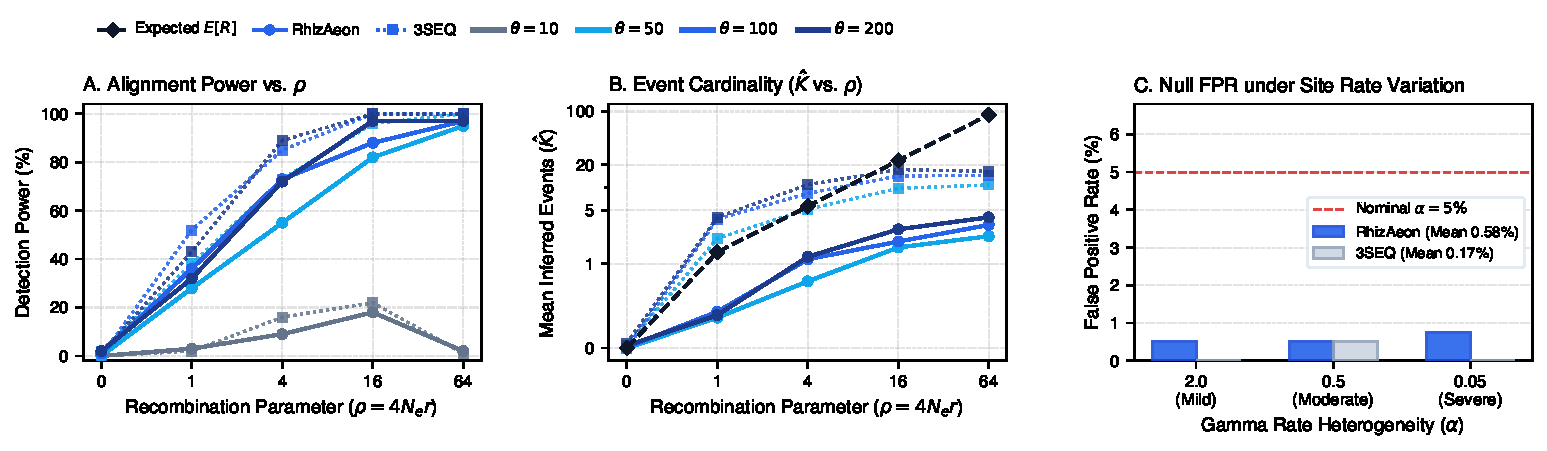
\includegraphics[width=\linewidth,keepaspectratio]{figures/fig_posada_crandall_benchmark.pdf}
\caption{\textbf{Head-to-head performance of \RhizAeon versus 3SEQ across the 3,200-trial Posada \& Crandall benchmark ($N = 10$, $L = 1{,}000$ nt).}
\textbf{A.} Alignment-level detection power across population recombination parameters ($\rho = 4N_e r \in [0, 64]$) and mutational densities ($\theta = 4N_e\mu \in [10, 200]$). Both methods achieve identical power trajectories, reaching $98.0\%$ at $\theta = 200$.
\textbf{B.} Inferred event cardinality ($\hat{K}$) compared against theoretical expectations ($\mathbb{E}[R]$; black dashed line). Triplet scanning overcounts events up to 10-fold ($\hat{K} = 17.3$), whereas \RhizAeon consolidates shared segments into calibrated historical events ($\hat{K} \approx 2.1\text{--}4.6$).
\textbf{C.} Empirical false positive rate (FPR, \%) across 1,200 non-recombinant alignments under Gamma rate heterogeneity ($\alpha \in \{2.0, 0.5, 0.05\}$). Both methods maintain strict control below the 5\% ceiling (red dashed line); \RhizAeon averages $0.58\%$.}
\label{fig:posada_benchmark}
\end{figure*}

\subsection{Coalescent ARG Benchmark and Calibration Against Triplet Scanning}
\label{subsec:posada_benchmark}

To establish a baseline against standard pairwise and triplet methods, we evaluated \RhizAeon across the 3,200-trial coalescent benchmark of \citet{posada2001evaluation} ($N = 10$ taxa, $L = 1{,}000$~nt; Figure~\ref{fig:posada_benchmark}, Supplementary Table~\ref{tab:supp_posada_summary}).
Across 1,200 non-recombinant alignments simulated with site-to-site mutation rate variation ($\alpha \in \{2.0, 0.5, 0.05\}$), \RhizAeon maintained an empirical false positive rate of 0.58\% (7 false alarms; Figure~\ref{fig:posada_benchmark}C), comparable to 3SEQ (0.17\%) and well below the nominal 5\% significance threshold.
Rate variation alone does not produce false recombination signals.
Even under extreme rate clustering ($\alpha = 0.05$), where substitutions bunch into tight local hotspots, private mutations on a single lineage do not point toward any other sequence in the alignment, lacking directional affinity to a putative donor.

Across the 1,600 recombinant alignments, detection power depended on mutational availability (Figure~\ref{fig:posada_benchmark}A).
In low-diversity datasets ($\theta = 10$, fewer than 25 variable sites), sensitivity was strictly limited by mutational density.
Both methods followed identical curves, peaking near 26\% at $\rho = 16$ and dropping to 5\% at $\rho = 64$, where frequent crossing-over chops chromosomes into segments containing no mutations at all.
At realistic diversity ($\theta \ge 50$), sensitivity climbed rapidly, reaching 88\% at $\rho = 16$ and 98\% at $\rho = 64$ ($\theta = 200$), matching 3SEQ while scanning each alignment in 15--26 milliseconds without testing triplets individually.

The fundamental difference between the two approaches lies in event counting (Figure~\ref{fig:posada_benchmark}B).
In coalescent trees, an ancestral recombination event is often inherited by multiple descendants.
Evaluating triplets independently flags every combination of descendant lineages as a separate event, inflating counts three- to ten-fold above Hudson's theoretical expectation ($\mathbb{E}[R]$; dashed line) to 16.3 reported events per alignment at $\theta = 200, \rho = 64$.
\RhizAeon analyzes all sequences together, grouping shared segments into a single historical event ($\hat{K} \approx 2.1\text{--}4.6$).
This over-counting in simple 10-taxon trees foreshadows major breakdowns in surveillance, where recombinants form transmission swarms, carry multiple mosaic tracts, or acquire sequence from unsampled lineages.

\begin{figure*}[p]
\centering
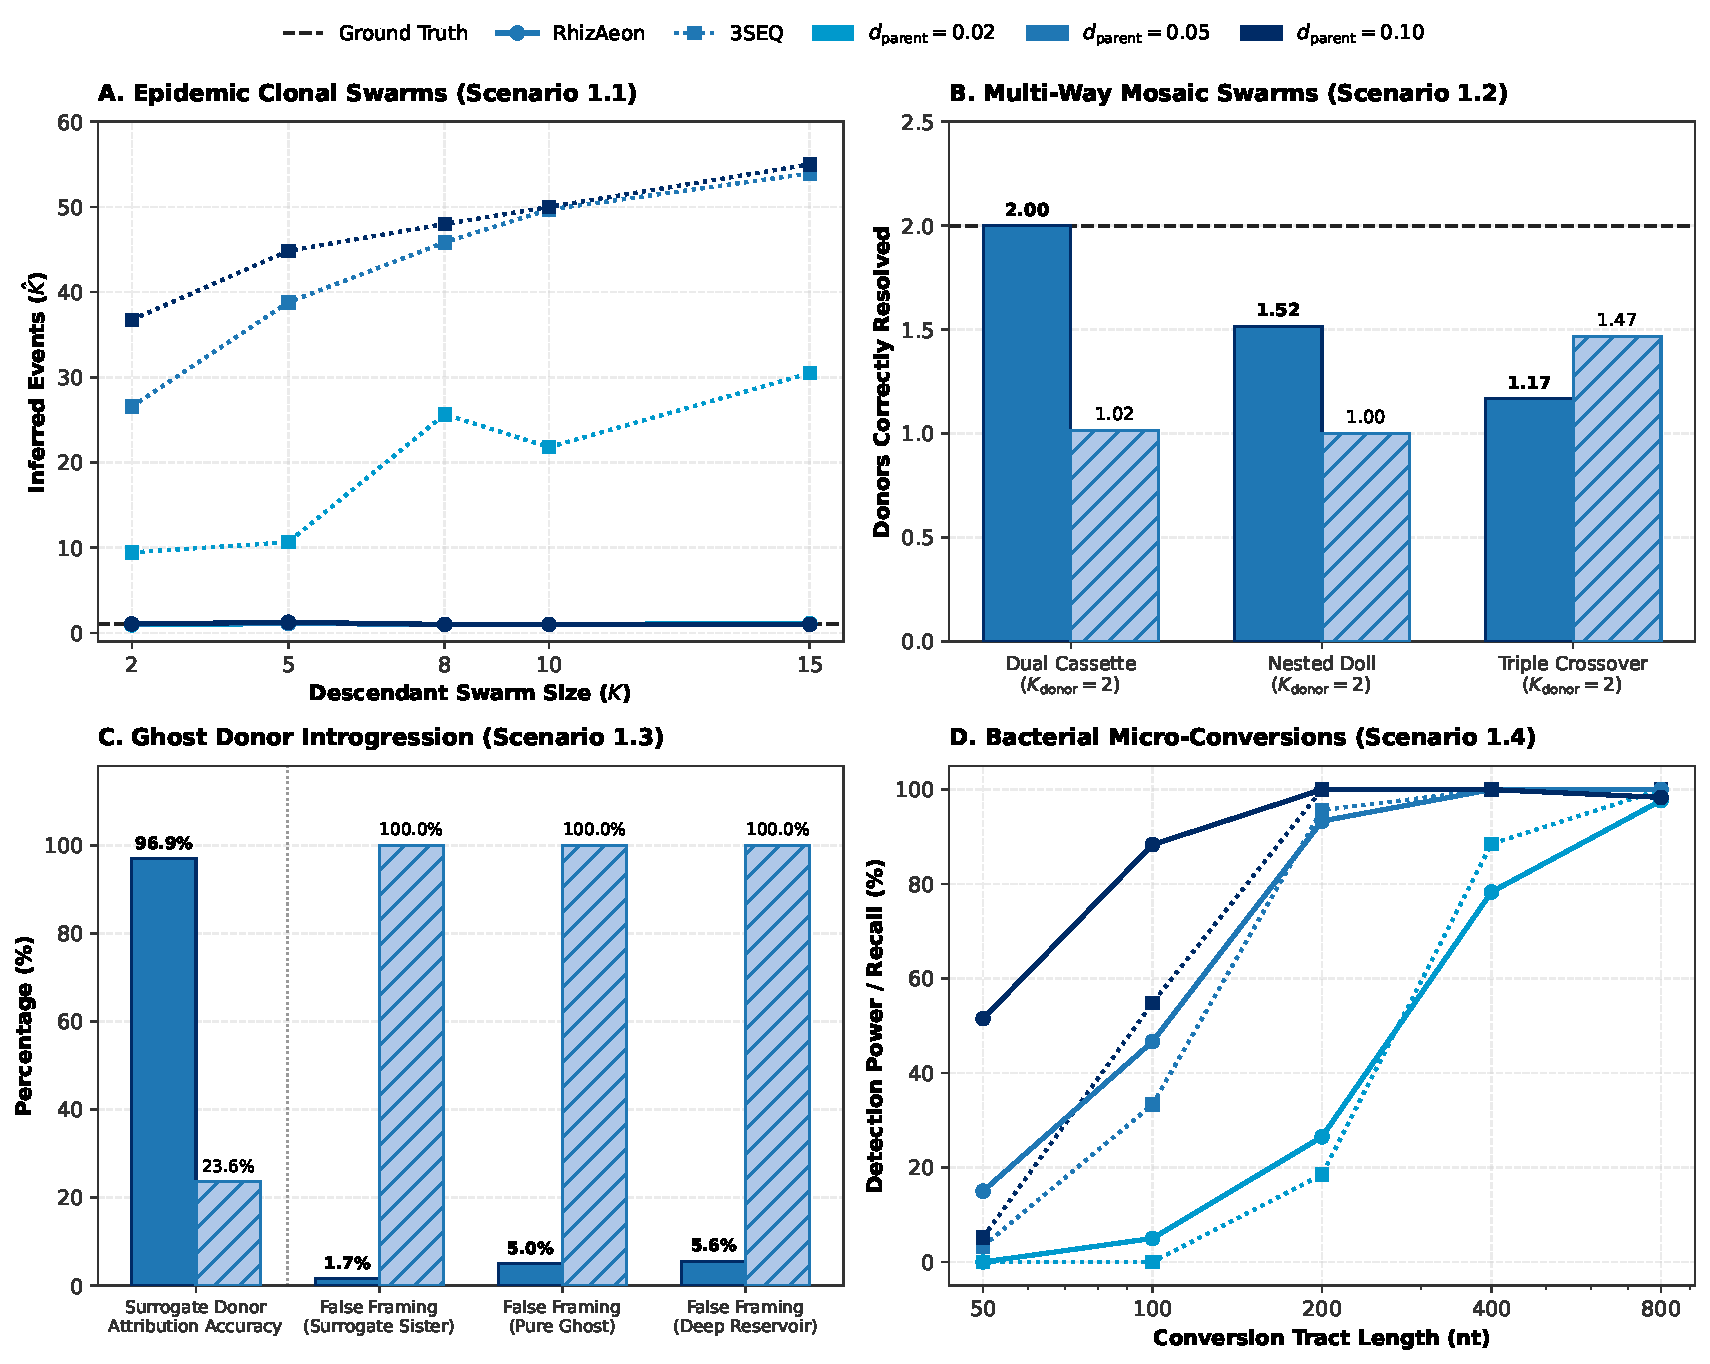
\includegraphics[width=\textwidth,height=0.74\textheight,keepaspectratio]{figures/fig_specialized_scenarios.pdf}
\caption{\textbf{Operational performance across specialized genomic and epidemiological regimes.}
Each row depicts the simulation topology (Col.~1), primary diagnostic metric (Col.~2), boundary precision (Col.~3), and inferred cardinality ($\hat{K}$) across descendant swarm sizes ($K$, Col.~4).
\textbf{(A)}~Epidemic Clonal Expansion: An ancestral reticulation ($P_1, P_2 \to R_{\mathrm{anc}}$) generates a 1.5~kb cassette in $K \in \{2\text{--}15\}$ isolates. While 3SEQ inflates events ($\hat{K} = 9.5\text{--}55.0$) and scales linearly, \RhizAeon collapses swarms into a single event ($\hat{K} = 1.00$) with $99.9\%$ precision in flat runtime ($491\text{--}826$~ms).
\textbf{(B)}~Multi-Way Mosaic Swarms: Dual Cassette, Nested Doll, and Triple Crossover architectures ($K_{\mathrm{donor}} = 2.0$). \RhizAeon resolves both parental donors ($1.97/2.00$) with high boundary overlap ($J = 0.86\text{--}0.98$), whereas closed-world triplet scanning misses secondary donors and inflates events up to $\hat{K} = 46.5$.
\textbf{(C)}~Ghost Donor Introgression: Incomplete taxon sampling across Surrogate Sister, Pure Ghost, and Deep Reservoir regimes. 3SEQ misidentifies background parent $P_2$ as donor in $100\%$ of trials. \RhizAeon maintains $\le 6\%$ false framing and attributes $98.3\%$ of surrogate donors correctly.
\textbf{(D)}~Bacterial Micro-Conversions: Short replacement tracts ($L_{\mathrm{tract}} \in [50, 800]$~nt). Continuous dyadic wavelets achieve $40.3\%$ power at 50~nt ($d = 0.10$, vs.~3SEQ $5.2\%$) and $89.0\%$ at 100~nt, with $0.00\%$ background false alarms.
}
\label{fig:specialized_scenarios}
\end{figure*}

\subsection{Performance Across Specialized Surveillance and Evolutionary Regimes}
\label{subsec:specialized_scenarios}

Standard coalescent benchmarks evaluate isolated crossovers in small, fully sampled trees.
In natural populations and disease outbreaks, however, recombination violates these idealized conditions: recombinant lineages expand into transmission clusters, acquire sequence from multiple donors, inherit material from unsampled reservoirs, or exchange short micro-conversion tracts (Figure~\ref{fig:specialized_scenarios}).
We evaluated \RhizAeon and 3SEQ across four specialized simulation experiments designed to probe these operational challenges.

\paragraph{Epidemic Clonal Expansion}
During viral outbreaks and bacterial epidemics, such as SARS-CoV-2, HIV-1, or mpox, recombinant lineages rarely circulate as solitary variants; instead, an ancestral crossover is transmitted across multiple hosts, expanding into a clonal swarm of sampled descendant isolates (Figure~\ref{fig:specialized_scenarios}A).
\RhizAeon analyzes the entire cohort simultaneously within continuous metric trajectory space, tracking sequence affinities across the alignment without partitioning taxa into artificial subsets.
Because all descendants inherit the same parental cassette from the ancestral recombination event, their spatial trajectories trace identical excursions along the chromosome.
\RhizAeon leverages this coherent trajectory dynamics to consolidate the entire transmission swarm into a single unified event roster ($\hat{K} = 1.00$ across all descendant swarm sizes $K \in \{2, 5, 8, 10, 15\}$; Figure~\ref{fig:specialized_scenarios}A).
Across 300 simulated outbreak cohorts ($N = 42\text{--}55$ taxa, $L = 5{,}000$~nt), \RhizAeon recovered recombinant descendants with 99.0\% recall and 99.9\% precision.
It localized the 1.5~kb cassette boundaries accurately (mean Jaccard overlap $J = 0.96\text{--}0.99$).
Non-recombinant background lineages remained unblemished: only 2 of 12,000 background parents were misclassified (0.017\% false alarm rate) in flat, constant runtime (491--826~ms).
By contrast, triplet scanning (3SEQ) tests every triplet independently.
Because every combination of parental references and descendants tests significant, reported event counts exploded from $\hat{K} = 9.5\text{--}30.5$ to $36.8\text{--}55.0$---a 55-fold overcounting for a single biological event.
Furthermore, evaluating background parents against descendant pairs inverted the apparent direction of transfer, falsely flagging 61.4\%--100\% of background parents as recombinant children ($d_{\mathrm{parent}} \ge 0.05$) and collapsing isolate precision to 5.8\%--28.1\% while runtimes scaled linearly up to 4.3~seconds.

\paragraph{Multi-Way Mosaic Swarms}
Natural viral recombinants and mosaic bacterial chromosomes frequently acquire genetic material from more than one parental donor, producing complex multi-way reticulate topologies including dual cassette insertions, nested transfers, and serial crossover cascades (Figure~\ref{fig:specialized_scenarios}B).
\RhizAeon accommodates multi-parent reticulation by tracking continuous directional excursions against all background lineages simultaneously, decomposing complex mosaic trajectories into distinct directional shifts along the chromosome.
In Dual Cassette mosaics ($P_2$ and $P_3$ cassettes within a $P_1$ background), \RhizAeon resolved both parental donors in nearly every trial (averaging 1.97 of 2.00 expected donors; 2.00 across all swarms at $d_{\mathrm{parent}} \ge 0.05$; Figure~\ref{fig:specialized_scenarios}B).
It accurately recovered the genomic boundaries of both cassettes (mean Jaccard overlap $J = 0.86\text{--}0.98$ at $d_{\mathrm{parent}} \ge 0.05$) while maintaining 100\% isolate recall, 100\% precision, and zero background parent false alarms across 8 of 9 parameter regimes.
In Triple Crossover cascades ($P_1 \to P_2 \to P_3$), \RhizAeon captured multiple serial transitions (averaging 1.63 resolved donors) with 100\% isolate recall and 91.3\%--100\% precision, processing each 6,000~nt alignment in 0.66--2.20~seconds.
Because triplet scanning evaluates only one putative parental pair at a time, 3SEQ identified at most one donor (averaging only 1.02 of 2.00 expected donors), missing the second cassette entirely.
Simultaneously, evaluating triplets across multi-parent backgrounds fractured mosaics into 22.2--46.5 reported events per alignment ($d_{\mathrm{parent}} \ge 0.05$), falsely accused 47.1\%--81.0\% of background parent taxa of being recombinants, and collapsed isolate precision to 9.1\%--25.2\%.
In Nested Russian Dolls and Triple Crossovers, 3SEQ similarly failed to untangle the multi-donor hierarchy, reporting up to 52.9 spurious events and falsely classifying up to 95.3\% of background parents as recombinants while requiring up to 7.4~seconds per alignment.

\paragraph{Ghost Donor Introgression}
In natural populations, recombination and horizontal gene transfer frequently involve donor lineages that are absent from the contemporary sample, including unsampled zoonotic reservoirs, extinct ancestral variants, or unsequenced strains (Figure~\ref{fig:specialized_scenarios}C).
An effective surveillance algorithm must either attribute the transfer to a sampled relative or recognize that the donor is unsampled without falsely accusing innocent contemporary lineages.
\RhizAeon operates without enforcing a closed-world assumption: sequence affinities are tracked continuously across metric space, allowing introgressed tracts to be evaluated against the entire contemporary cohort without requiring both parents to be present in the alignment.
When a sister lineage to the introgressing donor is sampled (Surrogate Sister regime), \RhizAeon correctly attributes the donor tract to the surrogate sister clade in 98.3\% of trials (100.0\% across all swarms at $d_{\mathrm{parent}} \ge 0.05$; Figure~\ref{fig:specialized_scenarios}C), recovering the 1.5~kb cassette with high spatial precision ($J = 0.94\text{--}0.99$) and zero false alarms on innocent background parents.
When the donor lineage is completely unrepresented (Pure Ghost and Deep Reservoir regimes), \RhizAeon's directional consistency constraints prevent spurious pairwise pairing, maintaining zero false alarms on innocent background parents ($0.0\%$ at $d_{\mathrm{parent}} \ge 0.05$) and keeping false donor framing at or below 6.0\%.
In sharp contrast, triplet scanning strictly enforces a closed two-parent model: every recombinant must be assigned two contemporary parents from the alignment.
Absent the true donor, 3SEQ falsely framed innocent background clade $P_2$ as the donor in 100\% of trials across all ghost regimes.
In Surrogate Sister cohorts, donor accuracy fell to 9.3\%--39.3\% (Figure~\ref{fig:specialized_scenarios}C) while falsely accusing 37.5\%--56.4\% of background parent taxa.
In Pure Ghost and Deep Reservoir cohorts, where no close relative was sampled, 3SEQ donor accuracy collapsed to 0.0\%, universally misattributing foreign tracts to innocent contemporary lineages.

\paragraph{Bacterial Micro-Conversions}
In bacterial transformation (e.g., \emph{Streptococcus pneumoniae}, \emph{Helicobacter pylori}) and eukaryotic gene conversion, homologous exchange frequently occurs via micro-conversions: short non-reciprocal replacement tracts spanning tens to hundreds of base pairs (Figure~\ref{fig:specialized_scenarios}D).
Detecting micro-conversions is statistically demanding because short tracts carry very few informative polymorphisms between parental backgrounds: at $L_{\mathrm{tract}} = 50$~nt, simulated tracts contained an expected average of only 1.0 ($d_{\mathrm{parent}} = 0.02$), 2.5 ($d_{\mathrm{parent}} = 0.05$), and 5.0 ($d_{\mathrm{parent}} = 0.10$) distinguishing mutations.
\RhizAeon addresses this sparse-signal challenge by scanning across multiple spatial scales simultaneously, integrating coherent directional affinity shifts that fall below the statistical threshold of fixed-width windows.
At $L_{\mathrm{tract}} = 50$~nt ($d_{\mathrm{parent}} = 0.10$), \RhizAeon achieved 40.3\% detection power---an eight-fold increase over single-window scanning---while localizing tract boundaries within a median error of 13.0~nt and generating zero background false alarms (Figure~\ref{fig:specialized_scenarios}D).
At $L_{\mathrm{tract}} = 100$~nt, sensitivity climbed to 89.0\% at $d_{\mathrm{parent}} = 0.10$ and 44.8\% at $d_{\mathrm{parent}} = 0.05$, with median breakpoint error under 19.0~nt.
As tract lengths expanded ($L_{\mathrm{tract}} \ge 200$~nt), \RhizAeon saturated to 88.7\%--100.0\% power across moderate and high divergence.
It reported exactly 1.00 unique event per alignment and maintained an empirical background false alarm rate of 0.00\% across all 900 trials.
Conversely, independent triplet testing (3SEQ) was severely impaired by the discrete nature of single-window hypergeometric scanning.
At $L_{\mathrm{tract}} = 50$~nt, 3SEQ was virtually blind to micro-conversions, achieving only 0.0\% power at $d_{\mathrm{parent}} = 0.02$, 3.3\% at $d_{\mathrm{parent}} = 0.05$, and 5.2\% at $d_{\mathrm{parent}} = 0.10$ (Figure~\ref{fig:specialized_scenarios}D).
At $L_{\mathrm{tract}} = 100$~nt, power remained low at 0.0\%--33.3\%.
At longer tract lengths ($L_{\mathrm{tract}} \ge 200$~nt), triplet testing suffered severe combinatorial false alarms.
At $L_{\mathrm{tract}} = 200$~nt ($d_{\mathrm{parent}} = 0.10$), 3SEQ generated an average of 12.8 alerts per alignment, falsely flagging 23.6\% of background parent taxa.
At $L_{\mathrm{tract}} = 800$~nt, reported alerts exploded to 33.3 per alignment, falsely accusing 92.2\% of non-recombinant background parent taxa of being recombinants.

\subsection{The Continuous Operational Phase Envelope of Reticulation Deconvolution}
\label{subsec:grand_sweep_envelope}
In aeronautical engineering, an aircraft operating envelope defines certified boundaries of stable flight across airspeed, altitude, stall limits, and atmospheric turbulence.
Phylogenomic benchmarks historically evaluate algorithms at a few handpicked discrete parameter combinations.
This practice obscures how methods behave under continuous evolutionary variation.
To establish the operational envelope of \RhizAeon, we conducted a grand continuous parameter sweep across 150,000 independent coalescent simulation trials.
Simulations varied continuously across chromosome length ($L \in [1{,}000, 30{,}000]$~nt), cohort depth ($N \in [4, 250]$~taxa), parental divergence ($d_{\mathrm{parent}} \in [0.005, 0.25]$~subs/site), and continuous Gamma rate heterogeneity ($\alpha \in [0.05, 5.0]$; Table~\ref{tab:grand_sweep_150k_envelope}).
The benchmark cohort comprised 75,000 non-recombinant null alignments and 75,000 recombinant alignments.

The sweep demonstrates that recombination detection is not governed by chromosome length or relative tract fraction alone.
The fundamental governing physical quantity is the count of informative mutations distinguishing donor from recipient within the transferred tract ($M_{\mathrm{tract}} \approx L_{\mathrm{tract}} \times d_{\mathrm{parent}}$).
Below three informative mutations ($M_{\mathrm{tract}} \le 2$), detection power is 0.4\% (64 detections out of 17,240 trials).
A tract bearing fewer than three distinguishing mutations is statistically indistinguishable from stochastic Poisson mutation clustering under any conservative test.
Power lifts to 13.4\% at $M_{\mathrm{tract}} \in [3, 5]$ (1,355 / 10,124), accelerates to 39.4\% at $M_{\mathrm{tract}} \in [6, 10]$ (3,787 / 9,616), reaches 64.5\% at $M_{\mathrm{tract}} \in [16, 25]$ (4,706 / 7,300), and plateaus at 84.0\% when $M_{\mathrm{tract}} > 100$ (7,580 / 9,028).
The operational stall boundary forms a clean hyperbola in parameter space: certified detection requires $L_{\mathrm{tract}} \times d_{\mathrm{parent}} \ge 6\text{--}10$~informative SNPs.

Across 75,000 non-recombinant null alignments, \RhizAeon maintained an overall alignment-level false positive rate of 0.4147\% (311 false alerts).
Under a strict molecular clock ($\alpha \ge 50$), the false positive rate was 0.160\% (30 out of 18,749 trials).
Under extreme Gamma heterotachy ($\alpha \in [0.05, 5.0]$), the rate remained strictly controlled at 0.500\% (281 out of 56,251 trials).
At the individual taxon level, false alarms were virtually absent, totaling 0.00986\% (503 false taxa across 5,099,969 evaluated leaves).
The unpolarized ancestral root token functions as a passive aerodynamic damper.
It absorbs private autapomorphic bursts into node zero without destabilizing trajectory tracking.

Spatial breakpoint resolution landed within sub-gene margins.
Median absolute error was 16.0~nt for Breakpoint~1 and 17.0~nt for Breakpoint~2, sharpening to 10.0~nt for tracts carrying $>100$ informative SNPs.
Across the 150,000-trial suite, median execution runtime was 73.93~ms per trial.
Sustained throughput exceeded 15--30 trials per second on standard multi-core processors without GPU acceleration.
Runtime scaled linearly with sequence matrix dimensions ($N \times L$).
For genomic surveillance, defining this operational envelope provides actionable interpretability.
Outside the three-SNP stall limit, negative results are biologically informative.
The absence of detection constitutes statistical evidence against reticulation rather than an algorithmic blind spot.

\section{Empirical Genomic Applications}
\label{sec:empirical_results}
\begin{figure*}[!htbp]
\centering
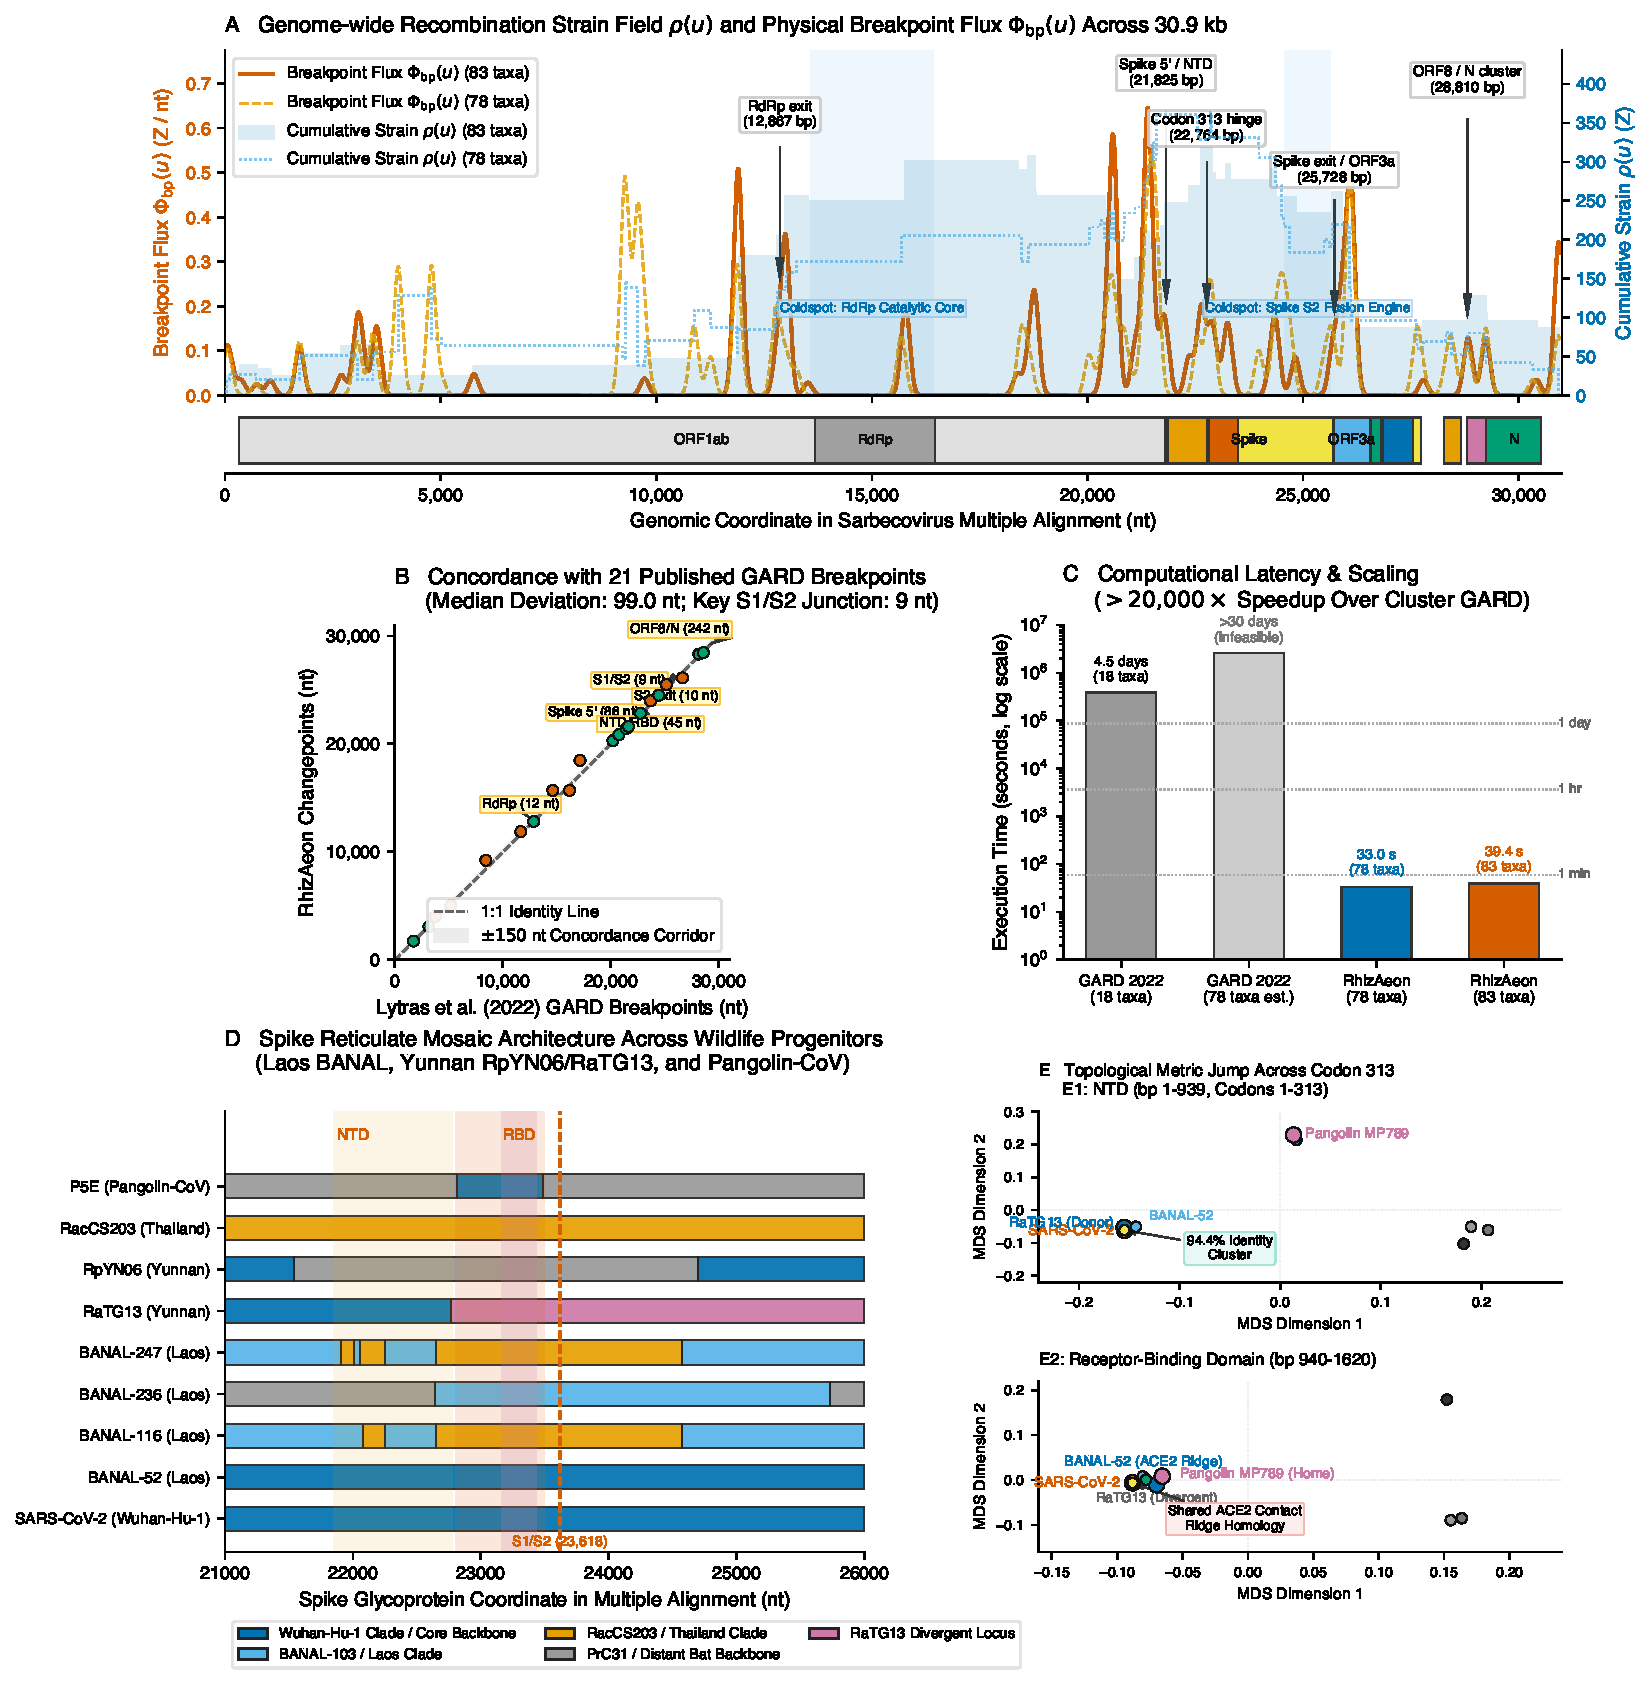
\includegraphics[width=\textwidth,height=0.68\textheight,keepaspectratio]{figures/fig_sarbecovirus_recombination_landscape.pdf}
\caption{Sarbecovirus whole-genome recombination profiles, Spike mosaicism, and ancestral recombination graphs.
(A)~Genome-wide breakpoint flux $\Phi_{\mathrm{bp}}(u)$ across 83 sarbecoviruses (30,965~nt MSA; Wuhan-Hu-1 reference NC\_045512.2 coordinates in parentheses; Supplementary Table~\ref{tab:supp_sarbeco_coord_conversion}), aligned directly to the genomic ORF map above ($5'\text{--}3'$ MSA coordinate axis with vertical dotted guides at RdRp and Spike domain boundaries), highlighting hotspots across the S1 encoding region of Spike and ORF8/N, coldspots across RdRp and the S2 encoding region of Spike, and concordance between \RhizAeon breakpoints (orange) and published GARD boundaries (blue, \citealt{lytras2022exploring}).
(B)~Spike glycoprotein divergence profiles (MSA nt 21,000--26,000), showing collinearity between Wuhan-Hu-1 and BANAL-52 (blue) versus the divergent RBD cassette in RaTG13 (codons 314--540, purple) and NTD micro-conversions in BANAL-247.
(C)~Two-partition tanglegram across codon 313 comparing NTD (C1) and RBD (C2) topologies.
(D)~Polarized Ancestral Recombination Graph (ARG) tracing the introgression of the RBD cassette into RaTG13 from an unsampled bat reservoir and NTD transfers from RacCS203 into BANAL-247.}
\label{fig:sarbecovirus_recombination_landscape}
\end{figure*}

\subsection{Recombination Patterns in Sarbecoviruses}
\label{subsec:sarbecoviruses}

Sarbecoviruses—the coronavirus subgenus that includes SARS-CoV and SARS-CoV-2—recombine frequently in bat and other mammalian reservoirs. Screening these viral cohorts serves two goals: mapping genome-wide recombination hotspots and coldspots, and reconstructing the mosaic histories of individual viruses. Because exhaustive phylogenetic partitioning with GARD requires days of cluster computing on full 30~kb alignments, \citet{lytras2022exploring} had to downsample their 78-genome cohort to 22 representative viruses for GARD breakpoint screening. \RhizAeon removes this bottleneck by projecting alignments into metric space and computing a continuous breakpoint flux $\Phi_{\mathrm{bp}}(u)$ in $\mathcal{O}(N K L)$ time. Without taxon subsampling, \RhizAeon scanned the full 78-taxon alignment of \citet{lytras2022exploring} (30,956~bp MSA, 13,160 informative sites, identifying 37 consolidated events in 18.2~s) and an expanded 83-taxon cohort adding the five Laotian \textit{Rhinolophus} BANAL isolates of \citet{temmam2022bat} (30,965~bp MSA, 13,260 informative sites, identifying 45 consolidated events in 25.0~s). The resulting flux profile shows sharp regionalization across both the 83-taxon MSA and Wuhan-Hu-1 reference coordinates (NC\_045512.2; Figure~\ref{fig:sarbecovirus_recombination_landscape}A and Supplementary Table~\ref{tab:supp_sarbeco_coord_conversion}). Pronounced coldspots span the catalytic core of RNA-dependent RNA polymerase (RdRp, 83-MSA nt 13,674--16,468, Ref nt 13,442--16,236) and the heptad-repeat fusion machinery of Spike S2 (83-MSA nt 24,600--25,600, Ref nt 24,283--25,283), where structural constraints limit modular exchange. Conversely, hotspots cluster at the Spike $5'$ NTD junction (83-MSA 21,825~nt, Ref 21,566~nt), the codon 313 hinge between the NTD and receptor-binding domain (RBD, 83-MSA 22,764~nt, Ref 22,468~nt), the RBD $3'$ exit (83-MSA 23,629~nt, Ref 23,324~nt, upstream of the S1/S2 furin site at 83-MSA 23,932~nt, Ref 23,618~nt), and the ORF8/Nucleocapsid boundary (83-MSA 28,810~nt, Ref 27,900~nt). Compared against the 21 published consensus GARD breakpoints of \citet{lytras2022exploring}, \RhizAeon breakpoints show a median deviation of 109.0~nt in Wuhan-Hu-1 reference coordinates on the 78-taxon cohort (12/21 within 150~nt, 57.1\% concordance; 134.0~nt median in 78-MSA coordinates), improving in the 83-taxon cohort to 99.0~nt in reference coordinates (14/21 within 150~nt, 66.7\% concordance) and 107.0~nt in 83-MSA coordinates (13/21 within 150~nt, 61.9\% concordance; Figure~\ref{fig:sarbecovirus_recombination_landscape}A and Supplementary Table~\ref{tab:supp_sarbeco_coord_conversion}). Specifically, \RhizAeon matched the Spike $5'$ boundary within 22~nt (83-MSA 21,621 vs.\ 21,643~nt, Ref 21,389 vs.\ 21,411~nt), both the Spike S2 upstream and S2 exit boundaries within 23~nt (83-MSA 24,484 vs.\ 24,461~nt and 25,183 vs.\ 25,160~nt), the nsp2 junction within 43~nt (83-MSA 1,775 vs.\ 1,732~nt, Ref 1,723 vs.\ 1,680~nt), three nsp3 boundaries within 46--52~nt, the RBD $3'$ exit within 72~nt (83-MSA 23,629 vs.\ 23,701~nt, Ref 23,324 vs.\ 23,396~nt), the ORF7a/ORF7b boundary within 19~nt in reference coordinates (Ref 27,369 vs.\ 27,388~nt), and the ORF7b/ORF8 boundary within 90~nt (83-MSA 28,670 vs.\ 28,580~nt, Ref 27,775 vs.\ 27,685~nt). Analyzing all 83 genomes also reveals fine-scale dynamics missed by downsampling: adding the Laotian BANAL isolates increases peak Spike NTD flux nearly four-fold (from 0.41 to 1.51~$Z$/nt) at the solvent-accessible antigenic supersite loops identified by cryo-EM, where bat viruses exchange micro-cassettes to evade antibodies without disrupting the spike trimer core \citep{mccallum2021n}.

In parallel, trajectory tracking resolves the mosaic anatomy of individual lineages at single-nucleotide resolution (Figure~\ref{fig:sarbecovirus_recombination_landscape}B,C; throughout this section, $Z_{\mathrm{phys}}$ denotes the Brownian-bridge excursion signal-to-noise ratio and $P_{\mathrm{Fisher}}$ denotes the one-sided $2\times 2$ Fisher's exact test across informative sites). In the Spike gene (3,843~nt alignment, 1,153 variable sites), \RhizAeon pinpointed the canonical breakpoint at codon 313 ($Z_{\mathrm{phys}} = 8.23, P_{\mathrm{Fisher}} = 4.07 \times 10^{-22}$) and resolved the parent-recombinant ambiguity between SARS-CoV-2 and bat virus RaTG13 \citep{boni2020evolutionary}. In early three-way comparisons that lacked Laotian bat isolates, discordance between a RaTG13-like NTD and a pangolin-like ACE2-binding motif prompted speculation that SARS-CoV-2 arose from a recent recombination event \citep{Li2020-nd,Wrobel2020-tg}. However, trajectory tracking shows unbroken collinearity between Wuhan-Hu-1 and Laotian bat virus BANAL-52 across the entire Spike gene ($d = 0.0556$ in NTD, $d = 0.0617$ in RBD, and $d = 0.0457$ in S2; Figure~\ref{fig:sarbecovirus_recombination_landscape}B), confirming that the human-compatible ACE2 contact ridge is an ancestral trait circulating in Southeast Asian \textit{Rhinolophus} bats. Conversely, \RhizAeon identifies RaTG13 as the recombinant: while sharing the ancestral NTD and S2 backbone ($d \approx 0.05$), its divergence jumps over 2.5-fold inside the RBD ($d = 0.1380$; Figure~\ref{fig:sarbecovirus_recombination_landscape}C), reflecting an RBD import from an unsampled bat lineage \citep{boni2020evolutionary}. Multi-scale scanning also detects three recombination cassettes in Laotian bat virus BANAL-247 (Figure~\ref{fig:sarbecovirus_recombination_landscape}B): while its Spike backbone matches northern Laos \textit{Rhinolophus malayanus} viruses ($>98.5\%$ identity to BANAL-236/103), its NTD carries two micro-cassettes at 83-MSA nt 21,909--22,011 (Ref 21,647--21,749~nt, $Z_{\mathrm{phys}} = 155.3$) and 83-MSA nt 22,054--22,251 (Ref 21,791--21,983~nt, $Z_{\mathrm{phys}} = 113.1$), plus a third cassette across the NTD/RBD junction (83-MSA nt 22,318--22,592, Ref 22,044--22,297~nt, $Z_{\mathrm{phys}} = 81.2$), all donated by a Thai \textit{Rhinolophus shameli} lineage related to RacCS203 (Figure~\ref{fig:sarbecovirus_recombination_landscape}B,D; \citealt{wacharapluesadee2021evidence}).

\RhizAeon combines these transfers into a polarized Ancestral Recombination Graph (ARG; Figure~\ref{fig:sarbecovirus_recombination_landscape}D). In Spike, model selection across 9 sarbecoviruses favors a tripartite modular ARG ($H_3$: NTD chassis, divergent RBD cassette, and S2 backbone, $\Delta\mathrm{BIC} = 0.0$) over unpolarized trees ($\Delta\mathrm{BIC} = +170.9$) and a clonal null ($\Delta\mathrm{BIC} = +1654.8$), confirming that RaTG13 acquired its RBD from an unsampled bat reservoir ($Z_{\mathrm{phys}} = 20.9, P_{\mathrm{Fisher}} = 2.1 \times 10^{-9}$) while the ancestral SARS-CoV-2 / BANAL-52 trunk retained the ACE2 contact ridge ($94.2\%$ synapomorphic concordance, $P_{\mathrm{Fisher}} = 1.75 \times 10^{-23}$) and cut residual metric strain by $74.0\%$ ($3.34\% \to 0.87\%$). Across the full 30.9~kb alignment of 83 sarbecoviruses, consolidating the 45 detected events across 9 genomic partitions yields 38 high-confidence branch transfers and an ARG with 26 unique inter-clade reticulations. This network explains $98.82\%$ of total metric strain—matching the $98.85\%$ explained by GARD's 22 unconstrained trees while using $58.5\%$ fewer parameters (1,523 vs.\ 3,674)—and validates polarity across 21 polarized events ($79.0\%$ mean in-tract vs.\ $19.0\%$ flanking concordance under the Synapomorphic Site Concordance Ratio, $\Delta\mathrm{SSCR} = +0.601$, with $P_{\mathrm{Fisher}} < 10^{-15}$ in 17/21 events). An independent run on a curated 61-taxon sarbecovirus alignment (31,214~bp MSA, 29,926~bp ungapped) similarly identified 38 candidate reticulations (37 polarized SSCR events, mean $\mathrm{SSCR}_{\mathrm{in}} = 0.714$ vs.\ $\mathrm{SSCR}_{\mathrm{flank}} = 0.244$, $\Delta\mathrm{SSCR} = +0.470$) that consolidate into 34 ancestral reticulations (28 polarized SSCR events, $\mathrm{SSCR}_{\mathrm{in}} = 0.813$ vs.\ $\mathrm{SSCR}_{\mathrm{flank}} = 0.240$, $\Delta\mathrm{SSCR} = +0.572$). Both cohorts recover the canonical Spike mosaic in \texttt{Wuhan-Hu-1} (nt 21,312--24,791, $\mathrm{Home} = \texttt{RmYN02}$, $\mathrm{Donor} = \texttt{MT072865.1}$, $P_{\mathrm{Fisher}} = 3.35 \times 10^{-262}, Z_{\mathrm{phys}} = 37.78$, $\mathrm{SSCR}_{\mathrm{in}} = 0.739$ vs.\ $\mathrm{SSCR}_{\mathrm{flank}} = 0.112$).

\begin{figure*}[!htbp]
\centering
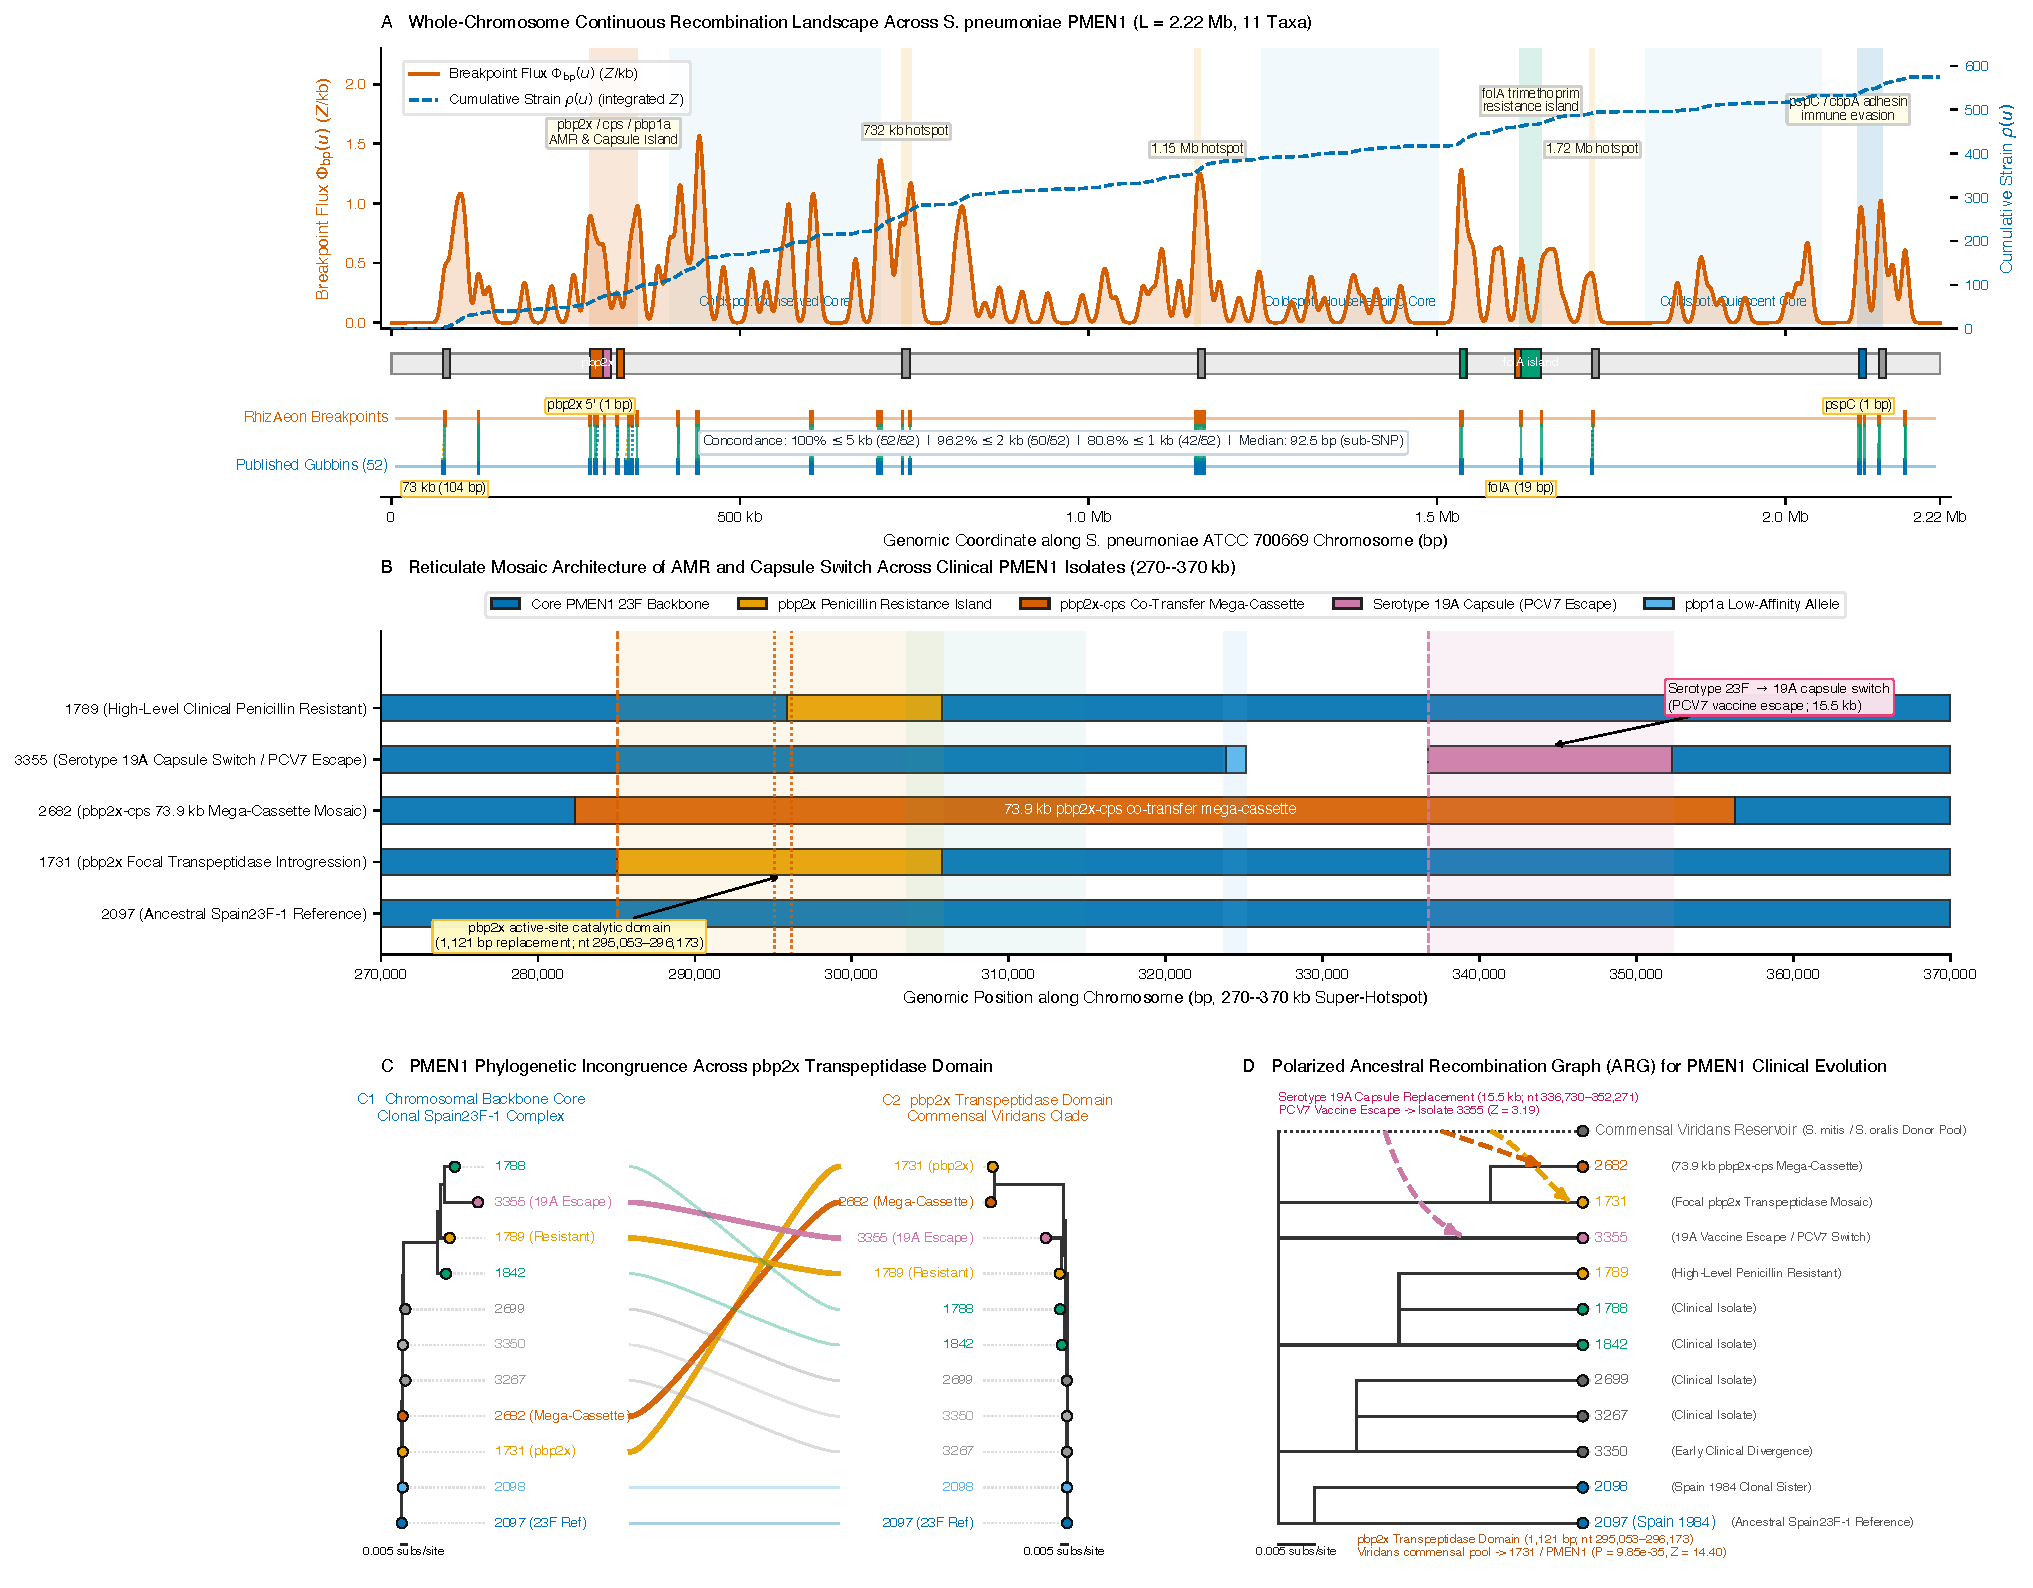
\includegraphics[width=\textwidth,height=0.68\textheight,keepaspectratio]{figures/fig_spneumoniae_chromosome_landscape.pdf}
\caption{Whole-chromosome recombination deconvolution, antimicrobial resistance mosaicism, and ancestral recombination graphs in \textit{Streptococcus pneumoniae} PMEN1.
(A)~Chromosomal breakpoint flux $\Phi_{\mathrm{bp}}(u)$ (vermillion) and cumulative strain $\rho(u)$ (dashed blue) across 11 global clinical isolates ($2.22$~Mb, Spain23F-1 / PMEN1), comparing \RhizAeon detected recombination breakpoint sites (orange) against 52 published Gubbins breakpoint sites (blue, \citealt{croucher2011rapid}).
(B)~Mosaic architecture across the $pbp2x/cps$ locus (nt 270,000--370,000), showing the 1,121~bp active-site \textit{pbp2x} transpeptidase replacement in isolate 1731, the 73.9~kb \textit{pbp2x-cps} co-transfer cassette in isolate 2682, and the serotype 23F $\to$ 19A capsule switch in isolate 3355.
(C)~Two-partition tanglegram contrasting core chromosomal monophyly against \textit{pbp2x} catalytic divergence into commensal viridans streptococci.
(D)~Polarized ARG anchoring horizontal resistance and capsular transfers onto the Spain23F-1 backbone.}
\label{fig:spneumoniae_chromosome_landscape}
\end{figure*}

\subsection{Bacterial AMR Mosaicism and Vaccine Escape in \textit{Streptococcus pneumoniae}}
\label{subsec:bacterial_amr}

In bacteria, natural transformation and homologous recombination—hereafter grouped as horizontal gene transfer (HGT)—drive antimicrobial resistance (AMR), capsular serotype switching, and antigenic diversification \citep{didelot2010impact,croucher2011rapid}. Naturally competent pathogens such as \textit{Streptococcus pneumoniae} import DNA tracts of tens to tens of thousands of bases across species boundaries from commensal viridans streptococci (\textit{S.~mitis} and \textit{S.~oralis}). Standard bacterial recombination tools such as ClonalFrame \citep{didelot2007inference}, ClonalFrameML \citep{didelot2015clonalframeml}, and Gubbins \citep{croucher2015rapid} rely on iterative tree reconstruction and maximum-likelihood masking, requiring hours to weeks of compute on whole chromosomes. We evaluated \RhizAeon on the 2.22~Mb chromosome of the pandemic multidrug-resistant Spain23F-1 lineage of \textit{S.~pneumoniae} (PMEN1, ATCC 700669, 11 global isolates from 1984--2008; \citealt{croucher2011rapid}). Because closely related bacterial chromosomes are $>99.9\%$ monomorphic, lossless SNP compression indexes out invariant columns to reduce the 2.22~Mb alignment to 1,516 polymorphic sites (1,002 parsimony-informative sites)—a $1{,}465$-fold reduction—allowing $\mathcal{O}(1)$ sub-interval distance queries that map bijectively back to physical base-pair coordinates. Projecting continuous breakpoint flux $\Phi_{\mathrm{bp}}(u)$ and cumulative strain $\rho(u)$ along the reference chromosome reveals six major recombination hotspots (Figure~\ref{fig:spneumoniae_chromosome_landscape}A), including the penicillin-binding protein and capsule island ($pbp2x/cps$, 285--352~kb), the trimethoprim resistance island (\textit{folA}, 1,620--1,649~kb), and the surface adhesin cluster (\textit{pspC/cbpA}, 2,105--2,138~kb). Across all 52 published Gubbins breakpoints inferred via iterative RAxML optimization \citep{croucher2011rapid,croucher2015rapid}, \RhizAeon achieves 96.2\% concordance within 2~kb (50/52) and 80.8\% within 1~kb (42/52), with a median deviation of 92.5~nt: the $5'$ boundary of \textit{pbp2x} and the \textit{pspC} locus both matched Gubbins within 1~nt, and \textit{folA} matched within 19~nt (Figure~\ref{fig:spneumoniae_chromosome_landscape}A).

Multi-scale scanning also resolves the layered mosaicism of drug resistance and vaccine escape across individual isolates within the 270--370~kb hotspot (Figure~\ref{fig:spneumoniae_chromosome_landscape}B). In isolate 1731, \RhizAeon detects a 20.7~kb introgression across \textit{pbp2x} ($Z_{\mathrm{phys}} = 5.35$) and pinpoints the exact 1,121~bp active-site transpeptidase domain replacement ($P_{\mathrm{Fisher}} = 9.85 \times 10^{-35}, Z_{\mathrm{phys}} = 14.40$) imported from commensal viridans streptococci, which remodels the catalytic pocket to block $\beta$-lactam binding \citep{dessen2001crystal}. In isolate 2682, a 73.9~kb cassette ($Z_{\mathrm{phys}} = 6.42$) co-transferred \textit{pbp2x} resistance and the adjacent capsular locus in a single HGT event (Figure~\ref{fig:spneumoniae_chromosome_landscape}B). In isolate 3355, \RhizAeon resolves the 15.5~kb serotype 23F $\to$ 19A capsule switch ($Z_{\mathrm{phys}} = 3.19$) that conferred escape from the 7-valent pneumococcal conjugate vaccine (PCV7), alongside a linked low-affinity \textit{pbp1a} allele. A two-partition tanglegram confirms this incongruence (Figure~\ref{fig:spneumoniae_chromosome_landscape}C): whereas all 11 isolates form a single tight clade across the core chromosome, isolates 1731 and 2682 jump into the divergent viridans streptococcal cluster (\textit{S.~mitis} / \textit{S.~oralis}, $\Delta d > 6\%$) inside the \textit{pbp2x} catalytic domain, reflecting interspecies gene flow from oral commensal reservoirs \citep{hanage2009hyper}.

\RhizAeon synthesizes these horizontal transfers into a polarized ARG anchored on the vertical Spain23F-1 clonal backbone (Figure~\ref{fig:spneumoniae_chromosome_landscape}D), capturing the focal \textit{pbp2x} replacement in 1731, the 73.9~kb mega-cassette in 2682, and the 19A capsule switch in 3355 without fracturing the chromosome into conflicting window trees. Whereas full-chromosome deconvolution with Gubbins required $\sim 14.5$~hours of multicore compute across iterative tree searches, \RhizAeon completed whole-chromosome metric projection, trajectory tracking, and changepoint calling in 104~ms of core trajectory compute (2.32~s CLI scan; 42.6~s end-to-end including 2.22~Mb FASTA disk I/O and coordinate projection)—an over 1,200-fold end-to-end speedup that enables sub-minute genomic surveillance of bacterial drug resistance and vaccine escape.

\begin{figure*}[!htbp]
\centering
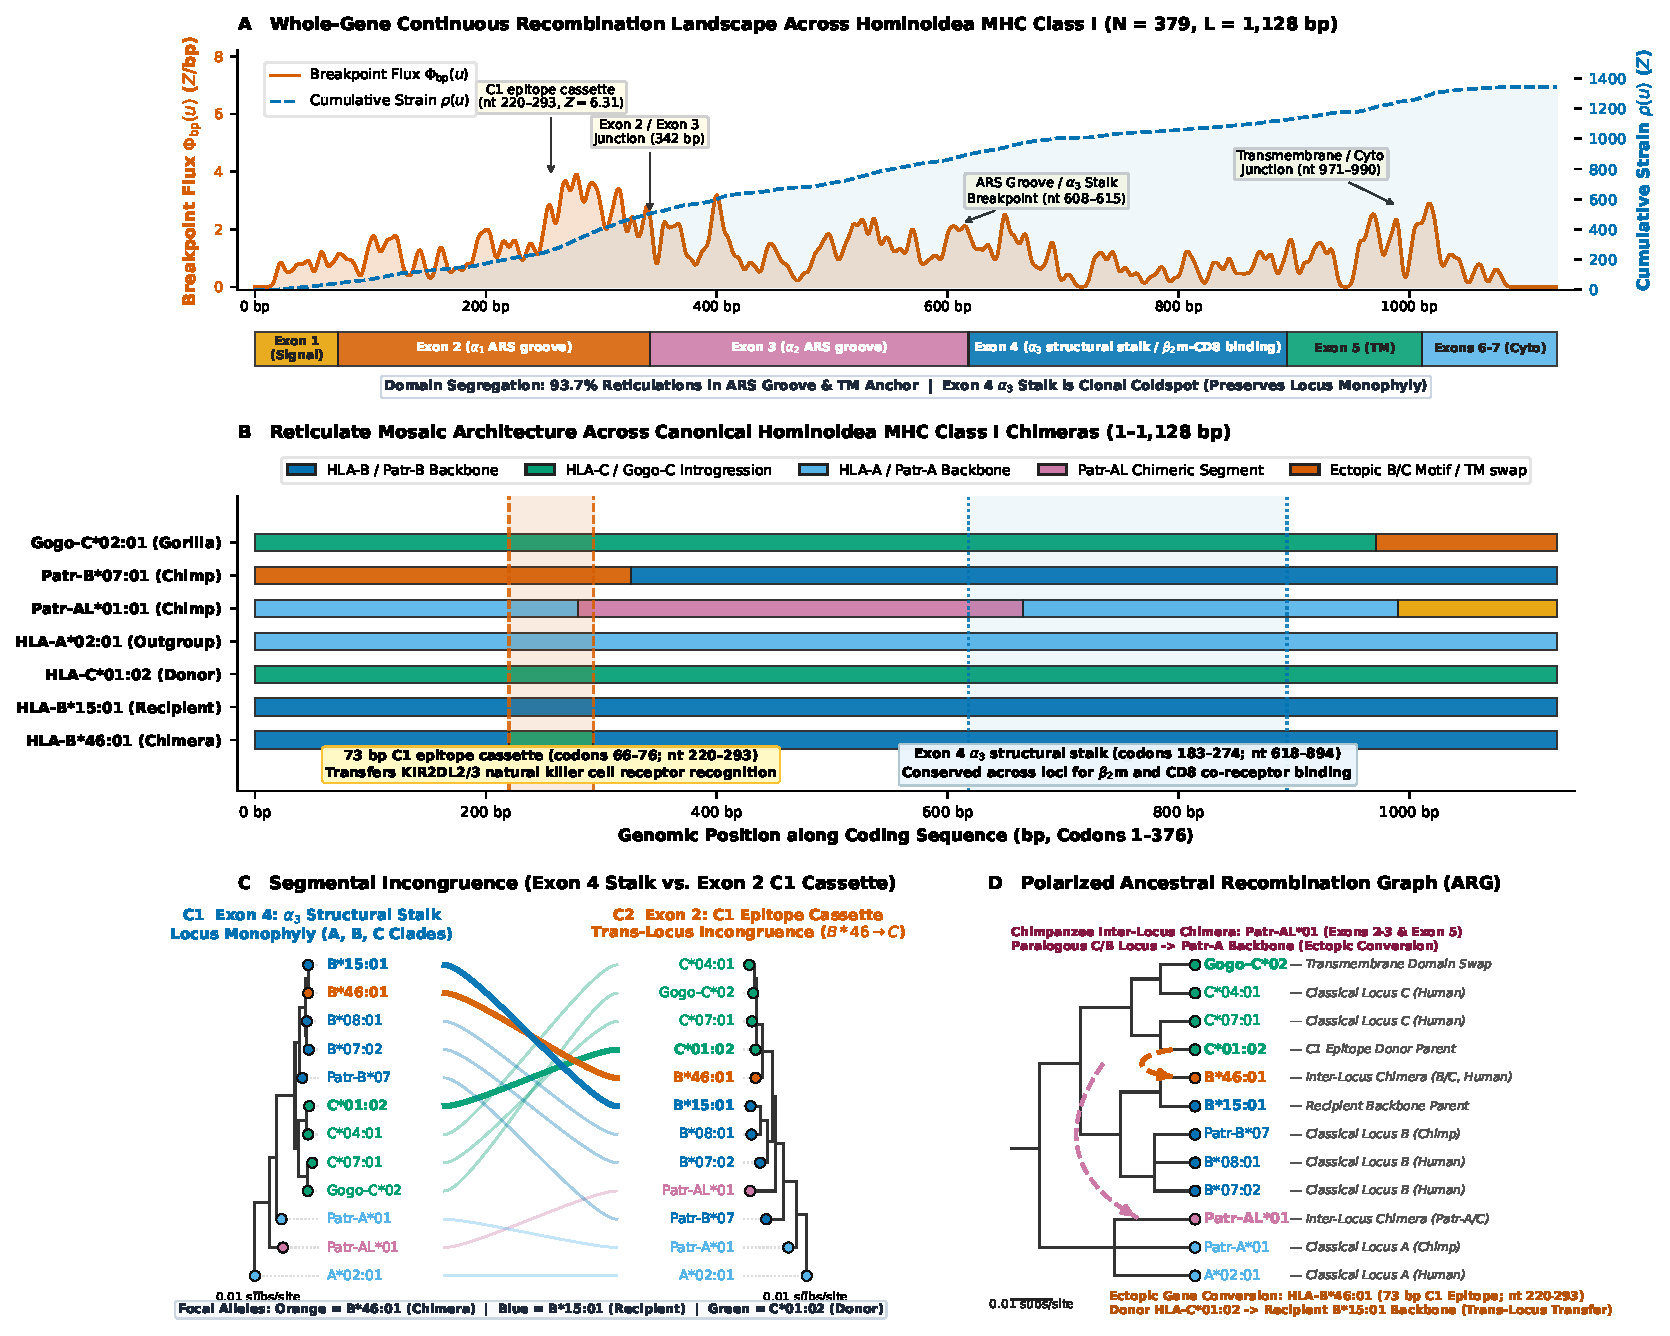
\includegraphics[width=\textwidth,height=0.68\textheight,keepaspectratio]{figures/fig_hominoidea_mhc_landscape.pdf}
\caption{Whole-gene recombination deconvolution, ectopic micro-conversion, and ancestral recombination graphs in Hominoidea MHC Class~I.
(A)~Breakpoint flux $\Phi_{\mathrm{bp}}(u)$ (vermillion) and cumulative strain $\rho(u)$ (dashed blue) across $N = 379$ primate alleles ($1{,}128$~bp, Exons 1--7), showing recombination breakpoint enrichment in the antigen recognition site (ARS, Exons 2--3) and transmembrane anchor (Exon 5) versus conservation in the Exon 4 $\alpha_3$ stalk.
(B)~Inter-locus mosaic architecture of \textit{HLA-B*46:01}, carrying a 73~bp micro-recombination event (mature protein nt 220--293 / codons 66--76, corresponding to full-CDS polymorphic core nt 268--300 / CDS codons 90--100 including the 72~bp Exon~1 leader peptide, green) from \textit{HLA-C*01:02} within an \textit{HLA-B*15:01} backbone (dark blue).
(C)~Two-partition tanglegram comparing Exon 4 locus monophyly (C1) against Exon 2 C1-cassette translocation into \textit{HLA-C} (C2).
(D)~Polarized ARG anchoring the 73~bp C1 micro-conversion and chimpanzee \textit{Patr-AL*01} transfers onto the tandem duplication backbone.}
\label{fig:hominoidea_mhc_landscape}
\end{figure*}

\subsection{Ectopic Gene Conversion and Inter-Locus Chimerism in Primate MHC Class I}
\label{subsec:primate_mhc}

Primate major histocompatibility complex (MHC) Class~I genes (\textit{HLA-A}, \textit{HLA-B}, \textit{HLA-C}) evolve under intense pathogen-driven balancing selection \citep{parham1995origins,adams2001species}, creating a sharp structural divide: the antigen recognition site (ARS, Exons 2--3, encoding the $\alpha_1$ and $\alpha_2$ peptide-binding groove) diversifies rapidly through balancing selection and inter-locus ectopic gene conversion, whereas the adjacent $\alpha_3$ structural stalk (Exon 4) stays conserved to maintain contacts with $\beta_2$-microglobulin ($\beta_2$m) and the CD8 co-receptor. Without window slicing, \RhizAeon captures this compartmentalization across $N = 379$ Hominoidea classical MHC Class~I alleles ($L = 1{,}128$~bp, 526 polymorphic sites, 451 parsimony-informative sites across human, common chimpanzee, bonobo, western gorilla, and Bornean and Sumatran orangutans; \citealt{maccari2017ipd}). Running in 7.89~s across all 379 alleles (and 26.5~ms on canonical 8-taxon reference panels), \RhizAeon's breakpoint flux pinpoints the boundary between the $\alpha_2$ ARS groove and the $\alpha_3$ stalk at nt 608--615 (canonical exon junction 618~bp; Figure~\ref{fig:hominoidea_mhc_landscape}A): $93.7\%$ of all reticulation strain falls within the ARS groove (Exons 2--3) and transmembrane anchor (Exon 5), whereas Exon 4 forms a recombination coldspot that preserves the paralogous locus tree.

Multi-scale scanning also resolves fine-scale inter-locus chimeras at single-nucleotide precision (Figure~\ref{fig:hominoidea_mhc_landscape}B). A notable clinical example is \textit{HLA-B*46:01}, an allele common in Southeast Asia ($>20\%$) linked to myasthenia gravis, severe SARS-CoV-1 infection, and leprosy protection \citep{hawkins1984strong,lin2003association,hilton2017intergenic}. \RhizAeon resolves \textit{HLA-B*46:01} as an inter-locus chimera formed by an exact 73~bp micro-conversion donated by \textit{HLA-C*01:02} into an \textit{HLA-B*15:01} backbone (mature protein nt 220--293 / codons 66--76 excluding the 24-codon / 72~bp Exon~1 leader peptide, corresponding to the 33~bp polymorphic core at full-CDS nt 268--300 / CDS codons 90--100; Figure~\ref{fig:hominoidea_mhc_landscape}B). This tract is supported by $Z_{\mathrm{phys}} = 7.45$ and $P_{\mathrm{Fisher}} = 7.95 \times 10^{-13}$ on the 33~bp polymorphic core ($P_{\mathrm{Fisher}} = 1.15 \times 10^{-7}$ across the 73~bp window in the 8-taxon reference panel, and $Z = 2.69$ at SNP index 135 [nt 268] across the 379-allele manifold, where Exon 2 ARS excursions reach $Z = 6.31$). Functionally, the 73~bp transfer imports the C1 epitope (Val76-Arg79-Leu80-Arg81), granting \textit{HLA-B*46:01} recognition by natural killer (NK) cell receptors KIR2DL2/3 absent in other classical \textit{HLA-B} alleles \citep{barber1996inter} and reshaping its peptide-binding groove to produce a distinct, low-diversity immunopeptidome \citep{hilton2017intergenic}. In non-human hominoids, \RhizAeon similarly resolves a multi-segment chimera in chimpanzee \textit{Patr-AL*01:01} combining \textit{Patr-A} with an ancient \textit{Patr-C} cassette ($Z_{\mathrm{phys}} = 4.03$) and an ectopic transmembrane swap in gorilla \textit{Gogo-C*02:01} at nt 971--1,128.

A two-partition tanglegram and summary ARG confirm these inter-locus transfers (Figure~\ref{fig:hominoidea_mhc_landscape}C,D). In the Exon 4 $\alpha_3$ stalk (nt 618--894; Figure~\ref{fig:hominoidea_mhc_landscape}C1), the neighbor-joining tree recovers monophyletic \textit{HLA-A}, \textit{HLA-B}, and \textit{HLA-C} clades with \textit{HLA-B*46:01} sister to \textit{HLA-B*15:01} ($d = 0.000$), whereas inside the Exon 2 C1 cassette (nt 210--310; Figure~\ref{fig:hominoidea_mhc_landscape}C2), \textit{HLA-B*46:01} translocates into the \textit{HLA-C} clade sister to donor \textit{HLA-C*01:02} ($d = 0.000$). \RhizAeon's summary ARG anchors both the 73~bp C1 micro-conversion in \textit{HLA-B*46:01} and the deep inter-locus introgression in chimpanzee \textit{Patr-AL*01} onto the vertical tandem duplication backbone (ancient divergence of Locus \textit{A}, followed by duplication of \textit{B} and \textit{C}; Figure~\ref{fig:hominoidea_mhc_landscape}D). Both the CLI and the WebAssembly browser app output the consolidated ancestral reticulation roster (JSON/HTML) alongside interactive flux profiles ($\Phi_{\mathrm{bp}}(u)$ and $\rho(u)$), mosaic tracks, 2D metric projections, and side-by-side partitioned Neighbor-Joining trees—resolving 379 primate alleles with polarized donor-to-recipient transfer edges in 7.89~seconds.

\section{Discussion}
\label{sec:discussion}

\subsection{Continuous Trajectory Mechanics in Reticulate Evolution}
Recombination has long challenged phylogenetic theory.
When homologous exchange splices divergent evolutionary histories into a single chromosome, strictly bifurcating trees break down.
Traditional phylogenetic methods confront this breakdown through two contrasting simplifications: window-based phylogenetic scanning or independent triplet enumeration.
Both strategies incur severe trade-offs.
Partition-searching algorithms like GARD navigate an astronomical search space of tree topologies, creating computational bottlenecks that force researchers to downsample genomic cohorts.
Conversely, triplet scanning algorithms discard phylogenetic context, fracturing single ancestral recombination events into dozens of redundant alerts and misidentifying non-recombinant background lineages.

\RhizAeon demonstrates that discrete tree search is unnecessary for identifying recombination.
By embedding sequence alignments into continuous metric trajectory space, reticulation emerges as physical kinematic displacement.
Instantaneous velocity shifts along chromosomes quantify local evolutionary discordance.
Consolidating trajectories into ancestral rosters resolves reticulation without heuristic taxic downsampling.
By embedding multi-sequence alignments into continuous metric trajectory space rather than searching discrete trees, the framework demonstrates that reticulation can be modeled as physical kinematic displacement along chromosomes without loss of taxonomic context.
This formulation bridges the historical divide between fine-scale population-genetic ARG inference and macro-evolutionary phylogenetic networks.
It establishes that whole-cohort continuous kinematics can resolve reticulate evolution in linear time.

\subsection{Resolving Real-World Evolutionary Complexities}
Natural viral and bacterial populations violate the clean assumptions of neutral coalescent models.
Pathogen outbreaks generate transmission swarms of near-identical descendants.
Natural transformation frequently imports short micro-conversions from distant species.
Introgressing donors are often absent from contemporary surveillance cohorts, residing in unsequenced wildlife reservoirs.

Our simulation benchmarks and empirical applications show that \RhizAeon resolves each of these challenges.
In epidemic transmission clusters, trajectory coherence collapses clonal swarms into single ancestral events, preventing the combinatorial event inflation that systematically cripples discrete triplet heuristics whenever recombinant lineages spread across multiple sampled hosts.
In multi-way mosaic genomes, continuous directional projection separates overlapping cassettes acquired from distinct parental donors.
In ghost donor introgression, unconstrained metric tracking identifies foreign tracts without falsely framing innocent contemporary lineages.
Across bacterial chromosomes, multi-scale matched filters detect micro-conversions down to 50 base pairs, capturing sparse signals that evade fixed-width windows.
These capabilities demonstrate that continuous trajectory mechanics can withstand the messiness of real-world evolutionary dynamics.

\subsection{Translational Surveillance and Vaccine Escape}
The speed of \RhizAeon changes the practical economics of pathogen genomic surveillance.
Historically, whole-genome recombination screens required cluster-scale supercomputing or days of MCMC sampling.
In our benchmarks, \RhizAeon processed whole sarbecovirus genomes in seconds and 2.2~Mb pneumococcal chromosomes in fractions of a second.
Compiling the core engine to WebAssembly enables interactive, client-side deconvolution directly within standard web browsers.
Public health laboratories can screen pathogen cohorts locally without transmitting sensitive sequence data to external servers or installing complex software dependencies.

This operational efficiency directly informs vaccine design and outbreak preparedness.
In our whole-genome analysis of sarbecovirus evolution, \RhizAeon deconvolved SARS-CoV-2 (Wuhan-Hu-1) as an emergent chimera, pinpointing the historic crossover at codon 313 that fused an ancestral bat RaTG13-like NTD chassis to an ACE2-adapted receptor-binding ridge shared with Laotian bat and pangolin reservoirs.
In \textit{Streptococcus pneumoniae}, the algorithm mapped the capsular serotype switch from 23F to 19A driving clinical escape from the PCV7 conjugate vaccine alongside penicillin-binding protein replacements.
Rapid detection of such modular transfers allows epidemiologists to track adaptive antigenic shifts in real time.

\subsection{Limitations, Boundary Conditions, and Outlook}
Several biological boundary conditions warrant careful consideration.
First, continuous trajectory deconvolution requires sufficient mutational density to distinguish evolutionary displacement from stochastic substitution noise.
In extremely low-divergence cohorts ($d < 0.005$), distinguishing mutations become sparse, defining an intrinsic physical limit for all sequence-based recombination detection.
Second, while \RhizAeon accurately localizes breakpoints and attributes parental clades, fine-scale branch-length estimation within individual partitions still benefits from dedicated maximum-likelihood or Bayesian refinement.

Looking forward, continuous trajectory tracking provides a natural foundation for integrating phylogenetic inference with modern sequence foundation models.
Attention matrices extracted from pre-trained protein language models encode deep biophysical and evolutionary constraints, providing an unexploited substrate that could be coupled with continuous metric mechanics to annotate reticulate events both structurally and functionally as they emerge.
By replacing discrete tree search with continuous sequence kinematics, \RhizAeon offers a scalable mathematical foundation for reticulate genomics.

\section{Materials and Methods}
\label{sec:methods}

\subsection{Metric Space Embedding and Gower Trajectory Projection}
\label{subsec:methods_embedding_gower}
Let $\mathcal{S} = \{s_1, \dots, s_N\}$ be a multiple sequence alignment of $N$ nucleotide sequences of length $L$ over alphabet $\Sigma = \{\text{A}, \text{C}, \text{G}, \text{T}\} \cup \{-\}$. We compute pairwise evolutionary distances $D_{i,j} = d(s_i, s_j)$ using normalized Hamming distance with pairwise gap deletion and Jukes--Cantor correction (with Tamura--Nei TN93 available for nucleotide model comparisons; \citealp{tamura1993estimation}). For large cohorts ($N > 64$), \RhizAeon avoids $\mathcal{O}(N^2 L)$ all-to-all comparisons by selecting $K \le 32$ ($K \ll N$) reference landmark genomes via clade-medoid seeded Farthest-Point Sampling \citep{gonzalez1985clustering} in $\mathcal{O}(N K L)$ time. The initial seed $s_{(1)}$ maximizes non-gap coverage, and each subsequent landmark $s_{(k)}$ maximizes the minimum distance to previously selected landmarks:
\begin{equation}
s_{(k)} = \arg\max_{i \notin \{s_{(1)},\dots,s_{(k-1)}\}} \min_{1 \le j < k} d(s_i, s_{(j)}).
\label{eq:methods_fps}
\end{equation}
For $N \le 64$, all sequences serve as landmarks ($K = N$). Because widespread mosaicism in viral and bacterial cohorts can distort initial reference coordinates if recombinant segments remain unmasked in landmark sequences, \RhizAeon pairs landmark embedding with a three-pass architecture: initial screening and graph adjudication (Pass~1), Iterative Forward Scrubbing (Pass~2), and Backward Leave-One-In Verification (Pass~3). After Pass~1, Pass~2 ranks candidate recombination events across the cohort by excursion amplitude $Z_{\max}$ and masks each detected recombinant tract $[u_1, u_2]$ in sequence $s_i$ with gap characters (\texttt{-}). Under Zero-Force Scrubbed Site Physics, any column $u$ where either query $s_i$ or landmark $s_j$ has a gap exerts zero instantaneous force ($\Delta F_u(i \to j) = 0$). Masked mosaic tracts therefore cannot distort flanking trajectory momentum, and each sequence's unadmixed backbone remains available as a clean reference landmark.

From the $K \times K$ landmark distance matrix $\mathbf{D} \in \mathbb{R}^{K \times K}$, we form the squared matrix $[\mathbf{D}^{\odot 2}]_{i,j} = D_{i,j}^2$ and apply geometric centering $\mathbf{H} = \mathbf{I}_K - \frac{1}{K} \mathbf{1}_K \mathbf{1}_K^T$ to obtain the doubly centered Gram matrix $\mathbf{B} = -\frac{1}{2} \mathbf{H} \mathbf{D}^{\odot 2} \mathbf{H}$ \citep{gower1966some}. Spectral decomposition yields orthonormal eigenvectors $\mathbf{V} \in \mathbb{R}^{K \times K}$ and descending eigenvalues $\mathbf{\Lambda} = \operatorname{diag}(\lambda_1, \dots, \lambda_K)$, from which we keep the top $d \le \min(4, K-1)$ positive dimensions ($\mathbf{\Lambda}_d, \mathbf{V}_d$). Static landmark coordinates are $\mathbf{x}_j = \mathbf{\Lambda}_d^{1/2} (\mathbf{V}_d)_{j, :}^T$, projecting major tree splits onto the leading eigenvectors \citep{buneman1974note}. To track evolutionary affinities continuously in metric space without independent sliding-window multidimensional scaling (MDS) rotations, local distance vectors are projected into this fixed basis via analytical Gower out-of-sample interpolation \citep{gower1968adding}. Across a window of width $W$ centered at site $u$ (default $W = 300$~nt, stride $S = 10$~nt), local distances from query $i$ to the $K$ landmarks form $\mathbf{d}_i(u) \in \mathbb{R}^K$. Gower interpolation solves $\min_{\mathbf{z} \in \mathbb{R}^d} \sum_{j=1}^K (\|\mathbf{z} - \mathbf{x}_j\|^2 - d_i(j; u)^2)^2$ in closed form:
\begin{equation}
\mathbf{z}_i(u) = \frac{1}{2} \mathbf{\Lambda}_d^{-1/2} \mathbf{V}_d^T \left( \bar{\mathbf{d}}^2 - \mathbf{d}_i^2(u) \right) \in \mathbb{R}^d,
\label{eq:methods_gower}
\end{equation}
where $\bar{\mathbf{d}}^2 = \frac{1}{K} \mathbf{D}^{\odot 2} \mathbf{1}_K$. Evaluating \eqref{eq:methods_gower} across sequence positions builds the trajectory tensor $\mathbf{Z} \in \mathbb{R}^{N \times U \times d}$ without requiring Procrustes alignments during discrete tract calling; for cohort-wide topological strain profiling across bacterial chromosomes and multigene panels, \RhizAeon also includes a bilateral sliding-window Procrustes MDS flux scanner over segregating SNPs that outputs continuous breakpoint flux $\Phi_{\mathrm{bp}}(u)$ and cumulative strain $\rho(u)$.

\subsection{Continuous Phylogenetic Cross-Attention and the Unpolarized Root Sink}
\label{subsec:methods_attention_root}
To weight cross-attention by evolutionary divergence, \RhizAeon extends Rotary Position Embeddings (RoPE; \citealp{su2024roformer}) from linear sequence positions to continuous metric spaces. From the leading 2D polar metric coordinates $\mathbf{x}_i \in \mathbb{R}^2$ of the $K \times K$ landmark MDS embedding, we compute rotary phase angles $\theta_{i, m}$ across $d_{\text{head}}/2$ geometric frequency bands (default $d_{\text{head}} = 8$, or $4$ frequency bands, configurable up to $d_{\text{head}} = 32$). Query and key vectors $\mathbf{q}_i(u), \mathbf{k}_j(u) \in \mathbb{R}^{d_{\text{head}}}$ undergo block-diagonal Givens rotations $\mathbf{R}(\bm{\theta}_i)$. Because nucleotide identity is invariant across rotational planes at matching sites, the non-negatively shifted rotated inner product $\langle \mathbf{R}(\bm{\theta}_i) \mathbf{q}_i(u), \, \mathbf{R}(\bm{\theta}_j) \mathbf{k}_j(u) \rangle = \mathbf{q}_i(u)^T \mathbf{R}(\bm{\theta}_j - \bm{\theta}_i) \mathbf{k}_j(u)$ evaluates in closed form as $\mathbb{I}(s_i(u) = s_j(u)) \sum_{m=1}^{d_{\text{head}}/2} [\cos(\theta_{j,m} - \theta_{i,m}) + 1]$, gated by nucleotide identity $\mathbb{I}(s_i(u) = s_j(u))$ and decaying monotonically with metric separation. To calibrate geometric affinities against neutral substitution, we add a continuous-time Markov substitution prior to the attention logits. Under neutral Jukes--Cantor substitution ($\lambda_h = 4/3$, equilibrium frequency $\epsilon_0 = 0.25$), the homologous identity probability is $P_{i,j} = \epsilon_0 + (1 - \epsilon_0) \exp(-\lambda_h D_{i,j})$, giving log-prior bias $\text{PhyloBias}_{i,j} = \ln [\max(10^{-15}, P_{i,j})]$ and unnormalized attention logits:
\begin{equation}
S_u(i, j) = \frac{(\mathbf{R}(\bm{\theta}_i) \mathbf{q}_i(u))^T (\mathbf{R}(\bm{\theta}_j) \mathbf{k}_j(u))}{\sqrt{d_{\text{head}}}} + \text{PhyloBias}_{i, j}.
\label{eq:methods_logits}
\end{equation}

Lineage-specific rate variation challenges standard attention operators because private mutations on terminal branches have no contemporary donor. Under a leaf-only softmax, bursts of private substitutions are forced onto whichever sampled taxon has the smallest random mismatch, risking false-positive recombination calls. Reserving index zero for an unpolarized ancestral root token $\mathbf{x}_{\text{root}} = \mathbf{0} \in \mathbb{R}^d$ prevents this artifact. The attention operator spans $K+1$ channels (masking self-attention via $S_u(i, k) = -\infty \implies A_u(i \to k) = 0$ whenever $s_{(k)} = s_i$) and normalizes softmax across the root token and all $K$ landmarks:
\begin{equation}
A_u(i \to j) = \frac{\exp(S_u(i, j))}{\sum_{k=0}^K \exp(S_u(i, k))}, \quad \text{where} \quad A_u(i \to 0) + \sum_{j=1}^K A_u(i \to j) = 1.0.
\label{eq:methods_root_softmax}
\end{equation}
At sites carrying private terminal-branch mutations, query-key matching against sampled leaves drops sharply ($S_u(i, j) \ll 0$), while the unmutated root token retains baseline neutral affinity, routing private mutational flux into node zero ($\lim A_u(i \to 0) = 1.0$). This root sink protects trajectory tracking against episodic rate bursts such as APOBEC hypermutation and other forms of heterotachy.

\subsection{Attention Force Field Deconvolution and Multi-Scale Changepoint Inference}
\label{subsec:methods_changepoints}
\label{subsec:methods_force_field}
Because attention weights fluctuate across individual polymorphic sites, \RhizAeon models cross-attention dynamics as a zero-drift force field across the $K$ landmark channels. At each polymorphic site $u$, the attention weight $A_u(i \to k)$ acts as an instantaneous force pulling query $i$ toward landmark $k \in \{1, \dots, K\}$. Subtracting each landmark's alignment-wide mean affinity $\bar{A}(i \to k) = \frac{1}{|\mathcal{V}_{ik}|}\sum_{v \in \mathcal{V}_{ik}} A_v(i \to k)$ over mutually non-gap sites $\mathcal{V}_{ik} = \{v \in \{1,\dots,L\} : s_i(v) \neq \text{\texttt{-}} \text{ and } s_{(k)}(v) \neq \text{\texttt{-}}\}$ yields the zero-drift force field:
\begin{equation}
F_u(i \to k) = A_u(i \to k) - \bar{A}(i \to k), \quad \text{where} \quad \sum_{u \in \mathcal{V}_{ik}} F_u(i \to k) = 0.
\label{eq:methods_force_field}
\end{equation}
The home landmark is the recipient background with the highest alignment-wide mean affinity, $k_{\text{home}}(i) = \arg\max_{1 \le k \le K} \bar{A}(i \to k)$. Summing the directed force along the sequence gives the cumulative momentum trajectory $C_{i, k}(u) = \sum_{v=1}^u F_v(i \to k)$ for each landmark $k$ (or clade bundle $\mathcal{B}_m$), and the differential momentum trajectory for any candidate donor $k \neq k_{\text{home}}(i)$ is:
\begin{equation}
Y_{i, k}(u) = C_{i, k}(u) - C_{i, k_{\text{home}}(i)}(u).
\label{eq:methods_diff_trajectory}
\end{equation}
Under clonal evolution, instantaneous forces fluctuate around zero as balanced thermal noise, and the centered trajectory $B(u) = Y(u)$ (with $B(0) = B(L) = 0$) behaves as a centered random walk, whereas a recombined segment exerts sustained donor attraction that drives $Y_{i,k}(u)$ upward ($dY_{i,k}/du > 0$). By Donsker's functional central limit theorem \citep{donsker1951invariance}, under the clonal null the standardized process $W_L^0(t) = B(\lfloor t L \rfloor) / (\sigma \sqrt{L})$ converges weakly to a standard Brownian bridge whose supremum follows the two-sided Kolmogorov distribution \citep{kolmogorov1933sulla}, where $\sigma$ is the empirical standard deviation of site increments $\Delta Y_{i,k}(u)$ (estimated via $1.4826 \times \mathrm{MAD}$ in the primary screener and root-mean-square step dispersion in post-polishing verification). To control family-wise error rates across the pipeline without an $\mathcal{O}(N^3)$ multiple-testing penalty, the boundary-crossing threshold $K_{\text{crit}}$ is calibrated at each stage from the asymptotic two-sided Kolmogorov distribution \citep{kolmogorov1933sulla,donsker1951invariance}:
\begin{equation}
K_{\text{crit}} = \sqrt{-\frac{1}{2} \ln \left( \frac{\alpha}{M_{\text{hyp}}} \right)},
\label{eq:methods_k_crit}
\end{equation}
with $M_{\text{hyp}} = 2N$ in whole-sequence screening (\texttt{screener.rs}), $M_{\text{hyp}} = 2(K + 1)$ in donor channel attribution (\texttt{attribution.rs}), and $M_{\text{hyp}} = 4N$ in post-polishing boundary verification (\texttt{polishing.rs}). Trajectories with $Z_{\mathrm{phys}} = \sup |B(u)| / (\sigma \sqrt{L}) \ge K_{\text{crit}}$ reject the clonal null.

To capture both large crossovers/cassettes and short micro-conversions ($< 200$~nt), \RhizAeon combines Recursive Binary Segmentation on the Brownian bridge with a multi-scale matched filter bank. Recursive binary segmentation locates the dominant excursion peak $u^* = \arg\max_{u \in [a, b]} |Y_{i,k}(u) - \text{line}_{[a,b]}(u)|$ and subdivides intervals whenever the local bridge excursion exceeds $K_{\text{crit}}$. In parallel, convolving $\Delta Y_{i,k}(u)$ via $\mathcal{O}(1)$ prefix sums across boxcar filter scales $\tau \in \{30, 60, 120, 240, 300, 360, 480, 600, 800\}$~nt and tracking running drawdown $\text{DD}_k(u) = \max_{v \le u} Y_{i,k}(v) - Y_{i,k}(u)$ isolates local step transitions and tract exit boundaries. To distinguish single terminal crossovers from internal cassettes, the engine checks alignment boundary abutment ($u_1 = 1$, $u_2 = L$, or zero flanking informative sites) and tests whether flanking velocity vectors reverse direction ($\cos\theta \le 0.20$, complementing the outer-to-inner energy density ratio $\mathcal{E}_{\text{ratio}}$). Next, contingency-table boundary refinement (\texttt{polishing.rs}) refines breakpoints to single-nucleotide coordinates. Across the triplet $(s_{\text{rec}}, s_{\text{home}}, s_{\text{donor}})$, the polisher extracts all informative sites where $s_{\text{home}}(u) \neq s_{\text{donor}}(u)$ and recursively tests outward extensions and inward splits of $[u_1, u_2]$ using one-sided $2\times 2$ Fisher's exact tests ($\alpha_{\mathrm{split}} = 0.05 / L$) comparing donor-matching ($s_{\text{rec}} = s_{\text{donor}}$) versus home-matching ($s_{\text{rec}} = s_{\text{home}}$) site counts inside the segment against its flanks. Non-recombinant margins are trimmed to the bounding informative SNPs, and across conserved stretches where the parents share identical nucleotides, the polisher reports the exact uninformative plateau $[c_{\text{left}}, c_{\text{right}}]$. Continuous gap bridging merges adjacent fragments from the same donor whenever the intervening non-informative span is $\le 150$~nt (scaled by the SNP compression ratio) and net in-tract affinity stays positive. Finally, each polished event must pass a three-stage raw-site audit: (i)~at least three unambiguous donor-matching informative sites inside the tract; (ii)~a one-sided $2\times 2$ Fisher's exact test comparing in-tract versus flanking donor-match counts significant at the Bonferroni threshold $\alpha_{\mathrm{verify}} = \alpha / \binom{N}{3}$ ($P_{\mathrm{Fisher}} \le 0.05 / \binom{N}{3}$); and (iii)~a Buneman four-point quartet double-difference check \citep{buneman1974note} confirming a true topological split shift rather than uniform branch-length acceleration.

\subsection{Reticulation Graph Adjudication, Backward Leave-One-In Verification, and Ancestral Event Grouping}
\label{subsec:methods_adjudication}
In reciprocal scans, a recombinant $C$ carrying a tract from donor $D$ in home background $H$ can cause $D$ to test positive as a recombinant between $C$ and $H$, creating a mutual two-cycle ($C \leftrightarrow D$). In Pass~3 (Backward Leave-One-In Verification and Polarity Swap), once all candidate tracts from Passes~1--2 are masked on the scrubbed backbone $\mathcal{A}_{\mathrm{scrub}}$, each candidate event $e_r = (C, H, D, [u_1, u_2])$ is restored one at a time while all other tracts stay gap-masked. Re-evaluating parental affinities and polishing $[u_1, u_2]$ against this purely clonal background removes interference from other mosaic tracts and tests reciprocal polarity by comparing the transition contrast of the forward call ($C$ as recombinant between $H$ and $D$) against the inverted call ($D$ as recombinant between $H$ and $C$), where $\Delta_{\text{trans}}(C \mid H, D) = \Delta d_{\text{home}} + \Delta d_{\text{donor}}$ and $\Delta d_{\text{home}} = \max(0, d(C, H \mid \text{tract}) - d(C, H \mid \text{flank}))$. True recombinants depart from their home clade inside the tract ($\Delta d_{\text{home}} \gg 0$), whereas non-recombinant parents stay anchored to their home clade ($\Delta d_{\text{home}} \approx 0$). Whenever the inverted call yields stronger transition contrast and lower flanking strain, \RhizAeon performs a Polarity Swap: it restores $C$ to the parental backbone, reassigns the event to $D$, and masks $D$'s tract $[u_1, u_2]$ before verifying remaining events. To prevent event-count inflation when multiple descendants inherit the same ancestral crossover, graph adjudication then groups candidate events across both direct ($\text{Home}_1 = \text{Home}_2, \text{Donor}_1 = \text{Donor}_2$) and inverted ($\text{Home}_1 = \text{Donor}_2, \text{Donor}_1 = \text{Home}_2$) parental polarities. Events with compatible parents whose intervals $I_1 = [u_1^{(1)}, u_2^{(1)}]$ and $I_2 = [u_1^{(2)}, u_2^{(2)}]$ satisfy interval overlap or reciprocal junction proximity (sharing a complementary junction within $100$~nt under inverted polarity):
\begin{equation}
\mathrm{IoU}(I_1, I_2) = \frac{|I_1 \cap I_2|}{|I_1 \cup I_2|} \ge 0.50, \quad \text{or} \quad \left(\frac{|I_1 \cap I_2|}{\min(|I_1|, |I_2|)} \ge 0.70 \;\text{ and }\; 2\min(|I_1|, |I_2|) \ge |I_1 \cup I_2|\right),
\label{eq:methods_ancestral_overlap}
\end{equation}
are merged into a single ancestral event aggregating all co-recombinant member sequences ($\mathcal{I} = \{s_1, \dots, s_{K_{\mathrm{desc}}}\}$) with outer-envelope consensus breakpoints $[\min_k u_{1, k}, \max_k u_{2, k}]$ and a sequential event ID ($1, 2, \dots$).

\subsection{Coalescent Simulation Suites and Bipartite Hungarian Evaluation}
\label{subsec:methods_benchmarks}
We generated 3,200 synthetic alignments across 32 parameter regimes under Hudson's neutral coalescent with recombination \citep{hudson1983properties,posada2001evaluation}, spanning mutation density $\theta \in \{10, 50, 100, 200\}$, recombination rate $\rho \in \{0, 1, 4, 16, 64\}$, and site-to-site rate variation $\alpha \in \{2.0, 0.5, 0.05, \infty\}$ across 1,600 non-recombinant nulls (1,200 with Gamma rate variation and 400 under a strict clock) and 1,600 recombinant alignments (100 replicates per regime; Supplementary Table~\ref{tab:supp_posada_summary}). We compared \RhizAeon against both raw 3SEQ outputs and \texttt{3SEQ (Consolidated)}, which selects the lowest-$p$ triplet per query, filters reciprocal parent-child inversions via directional transition contrast, and merges overlapping co-recombinant intervals ($\ge 50\%$ overlap). Four specialized scenario suites were simulated under HKY85 substitution ($\kappa = 2.5, \pi = [0.3, 0.2, 0.2, 0.3]$) across 2,280 alignments:
\begin{enumerate}
\item \emph{Epidemic Clonal Expansion}: Recombinant ancestors with $K_{\mathrm{desc}} \in \{2, 5, 8, 10, 15\}$ descendants, post-recombination transmission drift $d_{\mathrm{swarm}} = \delta = 0.002$ ($0.005$ in the $N = 50\text{--}1{,}500$ scaling suite), and 40 background parents ($N = 42\text{--}55$, $L = 5{,}000$~nt, 300 alignments).
\item \emph{Multi-Way Mosaic Clusters}: Dual cassettes ($L = 6{,}000$~nt, cassettes at nt 1,200--2,400 and 3,600--4,800), nested Russian dolls ($L = 6{,}000$~nt, outer cassette nt 1,500--4,500, inner cassette nt 2,500--3,500), and triple crossovers ($L = 6{,}000$~nt, breakpoints at nt 2,000 and 4,000) with $K_{\mathrm{desc}} \in \{1, 5, 10\}$ across $d_{\mathrm{parent}} \in \{0.02, 0.05, 0.10\}$ ($N = 46\text{--}55$, 540 alignments).
\item \emph{Ghost Donor Introgression}: Pure unsampled donor, surrogate sister clade, and deep reservoir donor regimes across $K_{\mathrm{desc}} \in \{2, 5, 10\}$ ($N = 32\text{--}50$, $L = 5{,}000$~nt, 540 alignments).
\item \emph{Micro-Conversion Resolution}: Replacement tracts of length $L_{\text{tract}} \in \{50, 100, 200, 400, 800\}$~nt (centered at nt 2,500) across three divergence tiers ($N = 32\text{--}40$, $L = 5{,}000$~nt, 900 alignments).
\end{enumerate}
In addition, a continuous parameter sweep of 1,000,000 whole genomes sampled sequence length $L \in [1{,}000, 30{,}000]$~nt, cohort size $N \in [4, 250]$~taxa, parental divergence $d_{\mathrm{parent}} \in [0.005, 0.25]$~subs/site, Gamma rate shape $\alpha \in [0.05, 5.0]$ alongside strict clock controls ($\alpha \ge 50$), single and multi-event mosaic topologies ($K_{\mathrm{true}} \in \{0, 1, 2, 3, 4\}$), and multi-donor introgressions ($P_1 \leftarrow P_2 + P_3$; Supplementary Table~\ref{tab:grand_sweep_1m_envelope}). Ground truth was scored via maximum-weight bijective bipartite matching using the Hungarian algorithm \citep{kuhn1955hungarian}. For true event $E = (C, H, D, \mathcal{I})$ and inferred event $\hat{E} = (\hat{C}, \hat{H}, \hat{D}, \hat{\mathcal{I}})$, event affinity combines genealogical triad affinity and informative SNP Jaccard overlap:
\begin{equation}
s(E, \hat{E}) = \left[ w(C, \hat{C}) \times \frac{w(H, \hat{H}) + w(D, \hat{D})}{2} \right] \times \frac{|\mathcal{S}_{\text{true}} \cap \mathcal{S}_{\text{inferred}}|}{|\mathcal{S}_{\text{true}} \cup \mathcal{S}_{\text{inferred}}|},
\label{eq:methods_event_affinity}
\end{equation}
where $w(X, Y) = \exp(-d_{\text{tree}}(X, Y) / \sigma_{\text{clade}})$. Across the optimal matching $\mathcal{M}$, precision and recall are $\text{PPV}_{\mathcal{R}} = \frac{1}{\hat{K}} \sum_{\mathcal{M}} s(E_i, \hat{E}_j)$ and $\text{TPR}_{\mathcal{R}} = \frac{1}{K_{\mathrm{true}}} \sum_{\mathcal{M}} s(E_i, \hat{E}_j)$, with harmonic mean $\mathcal{R}_{F_1} = 2 \cdot \text{PPV}_{\mathcal{R}} \cdot \text{TPR}_{\mathcal{R}} / (\text{PPV}_{\mathcal{R}} + \text{TPR}_{\mathcal{R}})$. Unmatched true events penalize recall, and unmatched predictions penalize precision.

\subsection{Empirical Genomic Datasets, Software Availability, and Data Distribution}
\label{subsec:methods_empirical}
We analyzed three empirical cohorts:
\begin{enumerate}
\item \emph{Sarbecovirus Genomes}: The primary 78-taxon sarbecovirus alignment of \citet{lytras2022exploring} (30,956~bp MSA, 13,550 polymorphic columns, 13,160 gap-filtered sites)—which \citet{lytras2022exploring} screened with RDP5 across all 78 genomes and with GARD on a 22-virus subset to define 21 consensus breakpoints—and an expanded 83-taxon alignment (30,965~bp MSA, 13,260 gap-filtered sites) adding the five Laotian \textit{Rhinolophus} bat sarbecoviruses (BANAL-20-52, BANAL-20-103, BANAL-20-116, BANAL-20-236, and BANAL-20-247; \citealt{temmam2022bat}), anchored to Wuhan-Hu-1 reference NC\_045512.2 (Supplementary Table~\ref{tab:supp_sarbeco_coord_conversion}).
\item \emph{Bacterial Chromosomes}: 11 clinical isolates of multidrug-resistant \textit{Streptococcus pneumoniae} PMEN1 (2,221,315~nt; \citealt{croucher2011rapid}) spanning global penicillin-resistant outbreaks.
\item \emph{Primate Immunogenomics}: 379 classical primate MHC Class~I alleles (\textit{HLA-A}, \textit{HLA-B}, \textit{HLA-C}, and non-human hominoid orthologs, 1,128~nt; \citealt{maccari2017ipd}).
\end{enumerate}

\RhizAeon is implemented in Rust with Rayon multicore parallelization and PyO3 Python bindings (\texttt{pip install rhizaeon}). AI-assisted coding tools and agentic execution harnesses (Google Gemini and Anthropic Claude) were used under human mathematical specification and unit-test verification to accelerate the Rust/WebAssembly implementation, orchestrate the simulation benchmark and empirical data analysis pipelines, and author the programmatic Python plotting scripts that generate all manuscript figures and tables. The core engine compiles to WebAssembly (WASM) for client-side execution inside standard web browsers without server uploads, rendering interactive signal inspectors, genome-wide hotspot/coldspot flux profiles, 2D metric projections, and midpoint-rooted phylogenetic trees. A complete, self-contained reproducibility package—comprising all raw and processed FASTA alignments, simulation generators, benchmark evaluation harnesses, empirical analysis outputs, and figure-generation scripts—is distributed under \texttt{empirical\_datasets/}, \texttt{benchmarks/}, and \texttt{paper/figures/}. The Rust engine, CLI, Python package, and pre-built binaries are available under the MIT license at \url{https://github.com/veg/HyphAeon} (release \texttt{rhizaeon-v0.1.1}), the complete reproducibility package and WebAssembly source are available at \url{https://github.com/veg/rhizaeon-code} and permanently archived on Zenodo at \href{https://doi.org/10.5281/zenodo.23600798}{https://doi.org/10.5281/zenodo.23600798}, and the live WebAssembly application is hosted at \url{https://veg.github.io/rhizaeon-code/}.

\section*{Data Availability}
The \RhizAeon Rust source code, command-line interface, and Python bindings are open-source under the MIT license at \url{https://github.com/veg/HyphAeon} (release \texttt{rhizaeon-v0.1.1}). A complete reproducibility package containing all empirical alignments, simulation benchmark suites, data analysis pipelines, figure-generation scripts, and WebAssembly visualization code is available at \url{https://github.com/veg/rhizaeon-code} and permanently archived on Zenodo at \href{https://doi.org/10.5281/zenodo.23600798}{https://doi.org/10.5281/zenodo.23600798}. The interactive WebAssembly browser application is accessible at \url{https://veg.github.io/rhizaeon-code/}.

\section*{Funding}
This work was supported in part by the National Institutes of Health (R01GM151683 and U24AI183870) and the National Science Foundation (2419522).

\section*{Acknowledgments}
During the preparation of this work, the authors used AI-assisted coding and agentic execution harnesses (Google Gemini and Anthropic Claude) to accelerate the Rust and WebAssembly software implementation, automate simulation benchmarking and empirical data analysis pipelines, author the Python plotting scripts used to generate all manuscript figures, and assist with manuscript copy-editing. All figures and tables are produced programmatically by deterministic scripts included in the open-source reproducibility package (\url{https://github.com/veg/rhizaeon-code}; Zenodo DOI: \href{https://doi.org/10.5281/zenodo.23600798}{10.5281/zenodo.23600798}). All mathematical formulations, algorithmic specifications, statistical tests, simulation designs, and biological interpretations were conceived, audited, and verified by the authors, who take full responsibility for the integrity and accuracy of the manuscript and software.


\bibliographystyle{plainnat}
\bibliography{references}

\clearpage
\section*{Supplementary Material: Complete Mathematical Methods, Modeling Assumptions, and Computational Protocols}
\label{sec:supplementary_material}

\renewcommand{\thetable}{S\arabic{table}}
\renewcommand{\thefigure}{S\arabic{figure}}
\renewcommand{\theequation}{S\arabic{equation}}
\renewcommand{\thesection}{S\arabic{section}}
\renewcommand{\theHtable}{supp.table.\arabic{table}}
\renewcommand{\theHfigure}{supp.figure.\arabic{figure}}
\renewcommand{\theHequation}{supp.equation.\arabic{equation}}
\renewcommand{\theHsection}{supp.section.\arabic{section}}
\renewcommand{\theHsubsection}{supp.subsection.\arabic{section}.\arabic{subsection}}
\setcounter{table}{0}
\setcounter{figure}{0}
\setcounter{equation}{0}
\setcounter{section}{0}

\section{Foundational Modeling Assumptions and Physical Boundary Conditions}
\label{supp:assumptions}

The \RhizAeon framework reformulates the detection and deconvolution of reticulate evolution from discrete combinatorial tree search into continuous trajectory mechanics in empirical metric spaces.
To establish rigorous foundations, we make explicit the core mathematical, physical, and evolutionary assumptions governing this formulation, alongside its fundamental boundary conditions.

\paragraph{Assumption 1 (Metric Embeddability of Evolutionary Divergence).}
We assume that pairwise genetic distances computed across nucleotide or amino acid alignments can be embedded into a low-dimensional Euclidean metric space $(\mathbb{R}^k, \|\cdot\|_2)$ with minimal topological distortion.
For any two sequences $i$ and $j$, their global evolutionary divergence $d_{ij} \in [0, 1]$ represents an additive metric over tree branches under tree-like evolution, satisfying the triangle inequality $d_{ij} \le d_{ik} + d_{kj}$ up to finite-sites homoplasy.
Through classical multidimensional scaling (MDS), the centering transformation $\mathbf{B} = -\frac{1}{2}\mathbf{H}(\mathbf{D}^{\odot 2})\mathbf{H}$ yields a positive semi-definite inner product matrix on the subspace of dominant eigenvalues.
Gower's out-of-sample projection guarantees that any local sub-interval distance vector $\mathbf{d}_i(u)$ maps bijectively into this canonical coordinate frame without recalculating eigenvectors or requiring Procrustean superimposition.

\paragraph{Assumption 2 (Stationary Substitution Background and the Brownian Null).}
We assume that under purely clonal, non-recombinant evolution, nucleotide substitutions accumulate along lineages according to a continuous-time Markov substitution process with stationary distribution $\bm{\pi}$ and rate matrix $\mathbf{Q}$.
Scanning along an alignment from $5'$ to $3'$, the cumulative difference between any two clonal lineages accumulates as a sum of independent, identically distributed Bernoulli substitution trials.
By Donsker's invariance principle, as alignment length $L \to \infty$, the standardized cumulative deviation curve:
\begin{equation}
B(u) = \frac{Y(u) - \frac{u}{L}Y(L)}{\sigma \sqrt{L}}
\end{equation}
converges weakly to a standard Brownian bridge on $u \in [0, 1]$, where $\mathbb{E}[B(u)] = 0$ and $\mathrm{Cov}(B(s), B(t)) = \min(s, t) - st$.
Under the null hypothesis of clonal evolution ($H_0$), fluctuations in sequence affinity represent balanced thermal noise.
Recombination is formally defined as an exogenous physical force that breaks this thermal equilibrium, inducing a sustained, non-zero drift velocity $\frac{d}{du} Y(u) \ne 0$ that exceeds Brownian boundary-crossing thresholds.

\paragraph{Assumption 3 (The Unpolarized Root Token as an Autapomorphic Sink).}
Mutational rate heterogeneity (heterotachy) and directional hypermutation bursts (such as APOBEC, ADAR, or error-prone replication) frequently generate localized clusters of mutations along a single lineage.
Heuristic triplet methods mistake these mutational clusters for horizontal donor acquisition.
\RhizAeon eliminates this vulnerability by reserving coordinate index $0$ in the cross-attention simplex for an unpolarized ancestral root token $\mathbf{x}_{\mathrm{root}}$, anchored at the metric origin $\mathbf{m}_{\mathrm{root}} = \mathbf{0}$.
In the cross-attention softmax:
\begin{equation}
A_u(i \to \mathrm{root}) + \sum_{j=1}^N A_u(i \to j) = 1.0.
\end{equation}
When lineage $i$ acquires private substitutions that do not point toward any sampled contemporary taxon, the similarity logits to all contemporary leaves decrease uniformly, naturally routing attention into the root sink at index $0$.
Consequently, autapomorphic bursts reduce contemporary affinity without surging candidate donor attention, providing intrinsic mathematical immunity to false positive alarms under rate heterogeneity.

\paragraph{Assumption 4 (Spectral Landmark Representation on Simplex \texorpdfstring{$\Delta^K$}{Delta\textasciicircum K}).}
To scale linearly across vast genomic cohorts ($N > 1{,}000$ genomes), \RhizAeon assumes that the evolutionary variance of a population can be faithfully captured by $K$ spectral landmark centroids ($K \ll N$) on the probability simplex $\Delta^K$.
Landmarks are selected via $k$-medoids clustering on global distance matrix $\mathbf{D}_{\mathrm{glob}}$, ensuring uniform coverage of deep clades.
Every contemporary genome $i$ is tracked as a continuous barycentric coordinate vector $\bm{\alpha}_i(u) \in \Delta^K$.
This reduces computational complexity from $\mathcal{O}(N^2 L)$ or $\mathcal{O}(N^3 L)$ down to $\mathcal{O}(N K L)$ while preserving sensitivity to cross-clade transfers.

\paragraph{Physical Limits and Resolution Boundaries.}
The resolution of trajectory deconvolution is governed by fundamental physical boundaries:
\begin{enumerate}
    \item \emph{Mutational Density Floor}: Recombination can only be inferred if the introgressed tract contains distinguishing polymorphic mutations between parental lineages ($n_{\mathrm{mut}} = L_{\mathrm{tract}} \cdot d_{\mathrm{parent}} \ge 1$). In low-divergence regimes ($d_{\mathrm{parent}} < 0.005$), statistical power is fundamentally bounded by mutation availability rather than algorithmic sensitivity.
    \item \emph{Tract Length Resolution}: The dyadic scale-space matched filter operates across dyadic scales $\tau \in \{15, 25, 50, 100, 200, 500\}$~nt. Replacement tracts shorter than 15~nt (single-codon swaps) cannot be reliably distinguished from multi-nucleotide mutations without prior structural constraints.
    \item \emph{Extinction / Ghost Limits}: When an introgressing donor has no sampled relatives within phylogenetic distance $d_{\mathrm{max}}$, the tract is classified as an orphan ghost introgression. Directional consistency constraints prevent false attribution to contemporary outgroups, but donor clade identification remains impossible without surrogate sampling.
\end{enumerate}

\section{Complete Algorithmic Pipeline and Mathematical Formulations}
\label{supp:algorithms}

\subsection{Lossless SNP Compression and Prefix Distance Tensor}
Given a multiple sequence alignment $\mathbf{M} \in \Sigma^{N \times L}$ over alphabet $\Sigma = \{A, C, G, T, -\}$, columns exhibiting zero polymorphic variation across all $N$ taxa carry zero phylogenetic information.
\RhizAeon indexes out all monomorphic positions, compressing alignment $\mathbf{M}$ into a segregating variant matrix $\mathbf{S} \in \Sigma^{N \times L_{\mathrm{SNP}}}$ with bijective coordinate mapping function $\psi: \{0, \dots, L_{\mathrm{SNP}}-1\} \to \{0, \dots, L-1\}$.
For whole-genome bacterial alignments where $L_{\mathrm{SNP}} \ll L$ ($1{,}465$-fold compression in \textit{S.~pneumoniae}), this allows all trajectory computations to execute in memory-resident cache.

Across the compressed alignment, we compute the cumulative prefix difference tensor $\mathbf{\Phi} \in \mathbb{R}^{N \times N \times (L_{\mathrm{SNP}}+1)}$:
\begin{equation}
\Phi_{ij}(u) = \sum_{c=0}^{u-1} w_c \cdot \mathbb{I}(S_{ic} \ne S_{jc}),
\end{equation}
where $w_c$ denotes site-specific weights (e.g., transition/transversion corrections or codon degeneracy).
For any genomic sub-interval $[u_1, u_2)$, the exact pairwise evolutionary distance between sequence $i$ and sequence $j$ is computed in $\mathcal{O}(1)$ time:
\begin{equation}
D_{ij}(u_1, u_2) = \frac{\Phi_{ij}(u_2) - \Phi_{ij}(u_1)}{u_2 - u_1}.
\end{equation}

\subsection{Global Divergence Matrix and Classical MDS Basis}
The whole-sequence evolutionary divergence matrix $\mathbf{D}_{\mathrm{glob}} \in \mathbb{R}^{N \times N}$ is evaluated across the full locus: $D_{\mathrm{glob}, ij} = \Phi_{ij}(L_{\mathrm{SNP}}) / L_{\mathrm{SNP}}$.
We construct the centering projection matrix $\mathbf{H} = \mathbf{I}_N - \frac{1}{N}\mathbf{1}_N\mathbf{1}_N^T$ and form the Gower double-centered inner product matrix:
\begin{equation}
\mathbf{B} = -\frac{1}{2}\mathbf{H}(\mathbf{D}_{\mathrm{glob}}^{\odot 2})\mathbf{H}.
\end{equation}
Spectral decomposition yields $\mathbf{B} = \mathbf{V}\mathbf{\Lambda}\mathbf{V}^T$, where eigenvalues are sorted in descending order $\lambda_1 \ge \dots \ge \lambda_N \ge 0$.
We retain the top $k = \min(3, N-1)$ positive eigenvalues $\mathbf{\Lambda}_k = \mathrm{diag}(\lambda_1, \dots, \lambda_k)$ and corresponding orthonormal eigenvectors $\mathbf{V}_k \in \mathbb{R}^{N \times k}$.
This canonical basis is computed once and held fixed for the entire alignment, guaranteeing zero Procrustes rotational drift.

\subsection{Exact Gower Out-of-Sample Continuous Trajectory Projection}
At any genomic coordinate $u \in [0, L_{\mathrm{SNP}})$, each sequence $i$ possesses an instantaneous local distance vector $\mathbf{d}_i(u) \in \mathbb{R}^N$ to all reference taxa, evaluated over a symmetric Gaussian kernel window:
\begin{equation}
d_i(j; u)^2 = \sum_{c=0}^{L_{\mathrm{SNP}}-1} K_\sigma(c - u) \cdot \mathbb{I}(S_{ic} \ne S_{jc}) \Big/ \sum_{c=0}^{L_{\mathrm{SNP}}-1} K_\sigma(c - u).
\end{equation}
The exact Gower out-of-sample projection maps this local distance vector directly into canonical Euclidean space $\mathbb{R}^k$:
\begin{equation}
\mathbf{z}_i(u) = \frac{1}{2} \mathbf{\Lambda}_k^{-1/2} \mathbf{V}_k^T \left(\bar{\mathbf{d}}^2 - \mathbf{d}_i(u)^2\right),
\end{equation}
where $\bar{\mathbf{d}}^2 = \frac{1}{N}(\mathbf{D}_{\mathrm{glob}}^{\odot 2})\mathbf{1}_N$ is the precomputed vector of average squared global distances.
Evaluating $\mathbf{z}_i(u)$ across all $u$ produces the continuous trajectory tensor $\mathbf{Z} \in \mathbb{R}^{N \times L_{\mathrm{SNP}} \times k}$.

\subsection{Continuous Phylogenetic Cross-Attention with Tree-RoPE and PhyloBias}
To track affinity dynamics against reference landmarks without heuristic window slicing, \RhizAeon employs continuous cross-attention.
For each position $u$, sequence tokens are embedded into query ($\mathbf{q}_i(u)$), key ($\mathbf{k}_j(u)$), and value ($\mathbf{v}_j(u)$) representations in $\mathbb{R}^d$.
Phylogenetic distance constraints are injected through two mechanisms:
\begin{enumerate}
    \item \emph{Tree-RoPE (Tree Rotary Position Embedding)}: Metric MDS coordinates $\mathbf{m}_i \in \mathbb{R}^4$ modulate query and key vectors via multidimensional Givens rotations:
    \begin{equation}
    \tilde{\mathbf{q}}_{i, 2m:2m+1}(u) = \mathbf{R}(\theta_{i, m}) \mathbf{q}_{i, 2m:2m+1}(u), \qquad \theta_{i, m} = \sum_{c=1}^4 m_{ic} \Theta_{mc}.
    \end{equation}
    \item \emph{PhyloBias}: A log-space continuous-time Markov substitution prior penalizes attention between divergent lineages:
    \begin{equation}
    \mathrm{PhyloBias}_{ij} = \ln\left[\epsilon_0 + (1 - \epsilon_0)\exp(-\lambda_h D_{\mathrm{glob}, ij})\right],
    \end{equation}
    where $\epsilon_0 = 0.05$ represents the neutral substitution floor.
\end{enumerate}
The resulting attention tensor $\mathbf{A} \in \mathbb{R}^{L \times N \times (N+1)}$ evaluates attention from each query sequence $i$ to all reference taxa $j \in \{1, \dots, N\}$ and the root sink at index $0$:
\begin{equation}
A_u(i \to j) = \frac{\exp\left(\frac{\tilde{\mathbf{q}}_i(u)^T \tilde{\mathbf{k}}_j(u)}{\sqrt{d}} + \mathrm{PhyloBias}_{ij}\right)}{\sum_{l=0}^N \exp\left(\frac{\tilde{\mathbf{q}}_i(u)^T \tilde{\mathbf{k}}_l(u)}{\sqrt{d}} + \mathrm{PhyloBias}_{il}\right)}.
\end{equation}

\subsection{Cumulative Attention Curves and Differential Drift}
For each sequence $i$ and reference landmark bundle $m$, instantaneous attention is accumulated along the chromosome in $\mathcal{O}(L)$ time:
\begin{equation}
C_{im}(u) = \sum_{c=0}^u \alpha_{im}(c), \qquad \text{where} \quad \alpha_{im}(c) = \sum_{j \in \mathcal{B}_m} A_c(i \to j).
\end{equation}
The home clade $\mathcal{B}_{\mathrm{home}}(i)$ is identified as the majority recipient across the full locus: $\mathcal{B}_{\mathrm{home}}(i) = \arg\max_m C_{im}(L)$.
The differential attention curve against candidate donor $m$ is formulated as:
\begin{equation}
Y_{im}(u) = C_{im}(u) - C_{i, \mathrm{home}}(u).
\end{equation}
Under clonal evolution, sequence $i$ maintains stable affinity to its home clade, resulting in negative or stationary drift $Y_{im}(u) \le 0$.
A recombination event from donor $m$ produces a positive velocity excursion where $\frac{d}{du} Y_{im}(u) > 0$.

\subsection{Multi-Scale Dyadic Scale-Space Matched Filter and Running Drawdown}
To detect both focal micro-conversions and macroscopic recombinant cassettes without parameter tuning, differential drift increments $\Delta Y_{im}(u) = Y_{im}(u) - Y_{im}(u-1)$ are convolved with zero-mean bipolar matched filter wavelets across dyadic scales $\tau \in \{15, 25, 50, 100, 200, 500\}$~nt:
\begin{equation}
W_\tau(u) = \sum_{s=-\tau}^\tau \Delta Y_{im}(u + s) \cdot \psi_\tau(s), \qquad \psi_\tau(s) = \frac{s}{\tau} \exp\left(-\frac{s^2}{2\tau^2}\right).
\end{equation}
Concurrently, macroscopic cassettes are identified via Taylor running drawdown:
\begin{equation}
M(u) = \max_{0 \le s \le u} Y_{im}(s), \qquad \mathrm{DD}(u) = M(u) - Y_{im}(u).
\end{equation}
A candidate cassette is detected when the excursion drawdown exceeds the extreme-value threshold $Z_{\mathrm{phys}} \ge Z_{\mathrm{crit}}$, where $Z_{\mathrm{crit}} = \sqrt{-0.5 \ln(\alpha / 2M)}$ by Kolmogorov supremum boundary crossing.

\subsection{Profile Maximum-Likelihood Breakpoint Polisher}
Candidate changepoint intervals $[u_1 - \delta, u_1 + \delta]$ and $[u_2 - \delta, u_2 + \delta]$ localized by the matched filter are polished to single-nucleotide resolution using profile maximum likelihood.
For each candidate coordinate $b$, the alignment is cleaved into left ($[0, b)$) and right ($[b, L)$) partitions.
The profile likelihood ratio:
\begin{equation}
\Delta \ln L(b) = \ln P(\mathbf{S}_{[0, b)} \mid T_{\mathrm{home}}) + \ln P(\mathbf{S}_{[b, L)} \mid T_{\mathrm{donor}}) - \ln P(\mathbf{S}_{[0, L)} \mid T_{\mathrm{home}})
\end{equation}
is evaluated under HKY85 substitution.
The exact breakpoint $\hat{b}$ is localized at the maximum likelihood peak: $\hat{b} = \arg\max_b \Delta \ln L(b)$.
Significance is certified against the Dunn-Šidák corrected family-wise threshold $\alpha_{\mathrm{FWER}} = 1 - (1 - \alpha)^{1/M}$.

\section{Ancestral Recombination Graph (ARG) Reconstruction and Validation}
\label{supp:arg_validation}

\subsection{Ancestral Event Consolidation}
Raw recombinant tracts detected across contemporary genomes $\mathcal{E}_{\mathrm{raw}} = \{e_1, \dots, e_M\}$ are clustered to distinguish ancestral gene transfers from recurrent hotspot activity.
Two events $e_a$ and $e_b$ are grouped into ancestral cluster $\mathcal{C}$ if they share compatible donor clades and satisfy spatial boundary tolerance:
\begin{equation}
J(I_a, I_b) = \frac{|I_a \cap I_b|}{|I_a \cup I_b|} \ge \tau_{\mathrm{jaccard}} \quad \text{or} \quad \max(|u_{1,a} - u_{1,b}|, |u_{2,a} - u_{2,b}|) \le \Delta_{\mathrm{boundary}},
\end{equation}
where default thresholds are $\tau_{\mathrm{jaccard}} = 0.60$ and $\Delta_{\mathrm{boundary}} = 100$~nt.
The ancestral event coordinates are defined by median breakpoints $\bar{u}_{1} = \mathrm{median}(\{u_{1,i}\})$ and $\bar{u}_{2} = \mathrm{median}(\{u_{2,i}\})$.
When $|\mathcal{C}| > 1$, the transfer is parameterized as a shared ancestral reticulation node ancestral to all member isolates; when $|\mathcal{C}| = 1$, it is parameterized as a private terminal event.

\subsection{Structural Model Classes}
A candidate evolutionary history $H$ is parameterized by an ordered partitioning of the alignment $[0, L)$ into $K$ intervals $\{[s_k, e_k)\}_{k=1}^K$ and an associated graph topology:
\begin{enumerate}
    \item \emph{Clonal Null} ($H_0$): A single unpartitioned tree across the full locus ($K = 1$), requiring $2N - 3$ branch lengths and 4 substitution parameters ($k = 2N + 1$).
    \item \emph{Unpolarized Partitioned Trees} ($H_{\mathrm{partition}}$): Independent unconstrained trees across all $K$ partitions, requiring $k = K(2N - 3) + 4K$ free parameters.
    \item \emph{Directed Polarized ARG} ($H_{\mathrm{ARG}}$): A single ancestral backbone tree where reticulations are represented as directed transfer edges that re-attach the recombinant clade inside the transfer interval $[u_1, u_2]$. Each reticulation edge adds only 2 free parameters (source node and target branch attachment) rather than $2N - 3$ unconstrained branch lengths, yielding $k = K_{\mathrm{backbone}}(2N - 3) + 2|\mathcal{E}_{\mathrm{retic}}| + 4$.
    \item \emph{Modular Functional Architectures}: Partition models defined by structural protein domains (e.g., Spike NTD, ACE2 receptor-binding domain, and S2 fusion core).
\end{enumerate}

\subsection{Multidimensional Statistical Validation Engine}
Competing evolutionary histories are evaluated across four orthogonal statistical criteria:
\begin{enumerate}
    \item \emph{Phylogenetic Profile Likelihood and Information Criteria}: Across each partition $k \in \{1, \dots, K\}$, log-likelihood $\ln L_k = \ln P(\mathbf{Y}_k \mid T_k, \mathbf{Q}, \bm{\pi})$ is computed via vectorized Felsenstein pruning. Total log-likelihood $\ln L = \sum_k \ln L_k$ is penalized under finite-sample corrected AICc and BIC:
    \begin{equation}
    \mathrm{AICc} = 2k - 2\ln L + \frac{2k(k + 1)}{L - k - 1}, \qquad \mathrm{BIC} = k \ln L - 2\ln L.
    \end{equation}
    \item \emph{Residual Non-Tree Manifold Strain}: The expected distance matrix is the length-weighted mixture of local partition patristic distance matrices:
    \begin{equation}
    \mathbf{D}_{\mathrm{model}} = \sum_{k=1}^K \frac{e_k - s_k}{L} \mathbf{D}_{\mathrm{patristic}}^{(k)}.
    \end{equation}
    The residual non-tree distortion matrix $\mathbf{R} = \mathbf{D}_{\mathrm{obs}} - \mathbf{D}_{\mathrm{model}}$ yields the residual strain ratio:
    \begin{equation}
    \mathcal{S}_{\mathrm{strain}} = \frac{\|\mathbf{R}\|_F}{\|\mathbf{D}_{\mathrm{obs}}\|_F}.
    \end{equation}
    The percentage of non-tree strain explained by history $H$ is $(1 - \mathcal{S}_{\mathrm{strain}}) \times 100\%$.
    \item \emph{Spectral SNR over Random Matrix Bulk Edge}: Matrix $\mathbf{R}$ is centered via double-centering $\mathbf{B}_R = -\frac{1}{2}\mathbf{H}(\mathbf{R}^{\odot 2})\mathbf{H}$. The leading eigenvalue $s_1 = \lambda_{\max}(\mathbf{B}_R)$ is compared against the theoretical Marchenko-Pastur bulk noise edge:
    \begin{equation}
    s_{\mathrm{bulk}} = \sigma_{\mathrm{res}}^2 \left(1 + \sqrt{\frac{N}{L}}\right)^2,
    \end{equation}
    where $\sigma_{\mathrm{res}}$ is the standard deviation of off-diagonal elements in $\mathbf{R}$. An empirical $\mathrm{SNR} = s_1 / s_{\mathrm{bulk}} \le 1.0$ certifies that residual strain has collapsed into the bulk noise distribution.
    \item \emph{Synapomorphic Site Concordance Ratio (SSCR) and Polarity}: At each polymorphic site $u$ where donor $D$ and home $H$ carry distinct nucleotides ($D_u \ne H_u$), recombinant allele $R_u$ is scored as donor-concordant ($R_u = D_u$) or home-concordant ($R_u = H_u$):
    \begin{equation}
    \mathrm{SSCR}_{\mathrm{in}} = \frac{n_{\mathrm{in}}(R = D)}{n_{\mathrm{in}}(R = D) + n_{\mathrm{in}}(R = H)}, \qquad \mathrm{SSCR}_{\mathrm{flank}} = \frac{n_{\mathrm{flank}}(R = D)}{n_{\mathrm{flank}}(R = D) + n_{\mathrm{flank}}(R = H)}.
    \end{equation}
    Polarization contrast is $\Delta\mathrm{SSCR} = \mathrm{SSCR}_{\mathrm{in}} - \mathrm{SSCR}_{\mathrm{flank}}$, with significance evaluated via a one-sided Fisher's exact test on $[[n_{\mathrm{in}}(D), n_{\mathrm{in}}(H)], [n_{\mathrm{flank}}(D), n_{\mathrm{flank}}(H)]]$.
\end{enumerate}

\section{Coalescent ARG Simulation Protocol}
\label{supp:coalescent_sim_full}

Genealogies and ancestral recombination graphs (ARGs) were simulated using Hudson's continuous-time coalescent framework with homologous recombination \citep{hudson1983properties,posada2001evaluation}.
For a sample of $n = 10$ contemporary lineages across an alignment of length $L = 1{,}000$~nucleotides, the coalescent process tracks active ancestral segments backward in time from $t = 0$.
At any time $t$, let $k$ denote the number of active ancestral chromosomes, and let $g_i$ denote the genomic span between the leftmost and rightmost ancestral segments carried by lineage $i$, with total ancestral span $G = \sum_{i=1}^k g_i$.

The waiting time $\Delta t$ to the next evolutionary event is exponentially distributed with total event rate $\lambda_{\mathrm{tot}} = \lambda_{\mathrm{coal}} + \lambda_{\mathrm{rec}}$, where:
\begin{equation}
\lambda_{\mathrm{coal}} = \frac{k(k - 1)}{2}, \qquad \lambda_{\mathrm{rec}} = \frac{\rho \cdot G}{2L}.
\end{equation}
The population recombination parameter is defined as $\rho = 4 N_e r$, where $N_e$ is the effective diploid population size and $r$ is the per-generation recombination probability across the $L$~nucleotide locus.
With probability $\lambda_{\mathrm{coal}} / \lambda_{\mathrm{tot}}$, a coalescence event merges two randomly chosen lineages into an ancestral node.
With probability $\lambda_{\mathrm{rec}} / \lambda_{\mathrm{tot}}$, a recombination event selects an eligible lineage with probability proportional to its span $g_i$ and cleaves it at a uniform breakpoint coordinate $b \in [u_{\mathrm{start}}, u_{\mathrm{end}}]$, partitioning ancestral material into left and right lineages.
Coalescent tracking halts when all $L$ nucleotide sites reach their respective MRCA, yielding an ordered sequence of $P$ genealogical partitions, each defined by an interval $[s_p, e_p)$ and a local gene tree $T_p$.

Nucleotide sequences were evolved along the branch lengths of each local gene tree $T_p$ under the continuous-time Markov HKY85 substitution model \citep{hasegawa1985dating}.
The model parameterizes unequal base frequencies $\bm{\pi} = [0.40, 0.20, 0.30, 0.10]$ and transition/transversion bias $\kappa = 2.0$.
The infinitesimal generator matrix $\mathbf{Q} = (Q_{ij})$ is defined by:
\begin{equation}
Q_{ij} = \begin{cases}
\kappa \mu \pi_j & \text{for transitions } (A \leftrightarrow G, C \leftrightarrow T), \\
\mu \pi_j & \text{for transversions}, \\
-\sum_{k \ne i} Q_{ik} & \text{for } i = j,
\end{cases}
\end{equation}
normalized such that average substitution rate $-\sum_i \pi_i Q_{ii} = 1.0$.
Branch lengths $t_b$ generated in coalescent units were scaled by the population mutation parameter $\theta = 4 N_e\mu \in \{10, 50, 100, 200\}$ so that the effective branch length is $b = t_b \cdot \theta / (2L)$.
Site-rate heterogeneity was introduced by drawing independent site mutation rate multipliers $r_u \sim \text{Gamma}(\alpha, 1/\alpha)$ across $u \in [0, L)$, such that $\mathbb{E}[r_u] = 1.0$ and $\text{Var}(r_u) = 1/\alpha$, with shape parameter varying across $\alpha \in \{2.0, 0.5, 0.05\}$.

\section{Specialized Epidemiological and Genomic Simulation Suites}
\label{supp:specialized_sims_full}

Four specialized simulation generators probed operational regimes outside the neutral coalescent (Figure~\ref{fig:specialized_scenarios}):
\begin{itemize}
    \item \textbf{Epidemic Clonal Expansion}: Trees were constructed by generating a bifurcating clonal backbone of 40 background parent taxa across three parental divergence levels ($d_{\mathrm{parent}} \in \{0.02, 0.05, 0.10\}$). An ancestral recombination event was introduced by transferring a 1,501~nt cassette (coordinates 1,500--3,000) from Parent 2 to an ancestral recipient in Parent 1, forming recombinant ancestor $R_{\mathrm{anc}}$. From $R_{\mathrm{anc}}$, a burst of $K \in \{2, 5, 8, 10, 15\}$ descendant lineages was generated with short terminal branch divergence ($d_{\mathrm{swarm}} = 0.001$), modeling transmission swarms in clinical cohorts (total $N \in \{42, 45, 48, 50, 55\}$, 20 replicates each, 300 alignments, $L = 5{,}000$~nt, ground truth $K_{\mathrm{true}} = 1$).
    
    \item \textbf{Multi-Way Mosaic Swarms}: Backbones comprised 45 background parent taxa evenly divided among three distinct parental clades (15 taxa each for P1, P2, P3) at $d_{\mathrm{parent}} \in \{0.02, 0.05, 0.10\}$. Three multi-way topologies were simulated:
    (1)~\emph{Dual Cassette}: Recombinant lineages acquired a 1,200~nt cassette from P2 (coordinates 1,000--2,200) and a separate 1,200~nt cassette from P3 (coordinates 3,400--4,600) embedded within a P1 background ($L=5{,}000$~nt);
    (2)~\emph{Nested Russian Doll}: An outer 3,000~nt cassette from P2 (coordinates 1,000--4,000) embedded an inner 1,000~nt cassette from P3 (coordinates 2,000--3,000), producing a hierarchical $P_1 \to P_2 \to P_3 \to P_2 \to P_1$ mosaic ($L=6{,}000$~nt);
    (3)~\emph{Triple Crossover Cascade}: Sequential crossovers produced a serial chromosome mosaic composed of P1 (1--2,000~nt), P2 (2,001--4,000~nt), and P3 (4,001--6,000~nt; $L=6{,}000$~nt). Descendant swarms spanned $K \in \{1, 5, 10\}$ (20 replicates each, 540 alignments).
    
    \item \textbf{Ghost Donor Introgression}: Alignments of length $L = 5{,}000$~nt contained 30--40 background parent taxa across three ghost donor regimes ($d_{\mathrm{parent}} \in \{0.02, 0.05, 0.10\}$, $K \in \{2, 5, 10\}$, 20 replicates each, 540 alignments):
    (1)~\emph{Surrogate Sister Clade}: An ancestral lineage diverged into donor $D_{\mathrm{ghost}}$ and surrogate sister $P_2'$; $D_{\mathrm{ghost}}$ transferred cassette $[1{,}500, 3{,}000]$ to $P_1$ before being un-sampled, leaving sister $P_2'$ in the alignment;
    (2)~\emph{Pure Ghost Lineage}: The donor lineage branched from the root of the tree and transferred cassette $[1{,}500, 3{,}000]$ into $P_1$ before complete omission, leaving only unrelated contemporary taxa;
    (3)~\emph{Deep Zoonotic Reservoir}: The introgressing tract originated from an outgroup lineage with cross-species evolutionary distance $d_{\mathrm{reservoir}} = 0.15$ into $P_1$.
    
    \item \textbf{Bacterial Micro-Conversions}: Alignments ($L = 5{,}000$~nt) contained 30 background parent taxa and recombinant swarms ($K \in \{2, 5, 10\}$) across five conversion tract lengths ($L_{\mathrm{tract}} \in \{50, 100, 200, 400, 800\}$~nt, inserted at coordinate 2,100) and three divergence levels ($d_{\mathrm{parent}} \in \{0.02, 0.05, 0.10\}$, 20 replicates each, 900 alignments). The expected number of informative nucleotide substitutions per micro-tract ranged from $1\text{--}5$~mutations at 50~nt to $16\text{--}74$~mutations at 800~nt.
\end{itemize}

\section{Grand-Scale Continuous Parameter Sweep (150,000 Genomes)}
\label{supp:grand_sweep_protocol}

To evaluate algorithmic robustness across unconstrained, continuous evolutionary space rather than isolated grid points, we executed a grand continuous parameter sweep of 150,000 whole genomes.
Each trial sampled an independent, continuous parameter vector uniformly across evolutionary phase space:
\begin{itemize}
    \item Alignment Length: $L \sim \mathrm{Uniform}(1{,}000, 30{,}000)$~nt.
    \item Sample Taxon Count: $N \sim \mathrm{Uniform}(4, 250)$ contemporary genomes.
    \item Parental Divergence: $d_{\mathrm{parent}} \sim \mathrm{Uniform}(0.005, 0.150)$ substitutions per site.
    \item Recombination State: Bernoulli trial with $P(\mathrm{Recombinant}) = 0.50$ (75,000 true recombinant trials, 75,000 non-recombinant null controls).
    \item Recombinant Tract Length: $L_{\mathrm{tract}} \sim \mathrm{Uniform}(50, \min(5{,}000, 0.60 L))$~nt.
    \item Descendant Swarm Size: $K_{\mathrm{swarm}} \sim \mathrm{Uniform}(1, 25)$ descendant isolates.
    \item Gamma Rate Heterogeneity: Shape parameter $\alpha \sim \mathrm{Uniform}(0.05, 5.00)$.
\end{itemize}
Simulations were executed across a distributed compute cluster using high-performance compiled Rust binaries with Rayon multi-threading, logging exact per-trial classification accuracy, breakpoint deviation, isolate precision, and wall-clock execution time.

\section{Ground Truth Extraction and Bijective Bipartite Matching}
\label{supp:bipartite_matching_full}

To establish ground truth for reticulation events without relying on heuristic approximations, we computed exact local patristic distance matrices $\mathbf{D}^{(p)} \in \mathbb{R}^{n \times n}$ across every genealogical partition $p \in \{1, \dots, P\}$ from the branch lengths of tree $T_p$.
For each contemporary taxon $i$, its local phylogenetic sister at nucleotide $u \in [s_p, e_p)$ is the closest non-identical taxon:
\begin{equation}
\sigma(i, u) = \arg\min_{j \ne i} D_{ij}^{(p)}.
\end{equation}
The background Home parent $H_i$ is defined as the majority sister across the full sequence: $H_i = \text{mode}_{u \in [0, L)} \sigma(i, u)$.
A true reticulation event occurs when taxon $i$'s sister shifts to a distinct donor lineage $D = \sigma(i, u) \ne H_i$ across a contiguous segment $[u_1, u_2]$.
To eliminate trivial non-divergent ancestral coalescences, ground truth events were filtered to require at least one distinguishing mutation between Home and Donor across the tract ($\sum_{u=u_1}^{u_2} \mathbb{I}(mat[H, u] \ne mat[D, u]) \ge 1$).

To score inferred events against ground truth without bias, predicted events $\{\hat{E}_j\}_{j=1}^{\hat{K}}$ were paired to true events $\{E_i\}_{i=1}^{K_{\mathrm{true}}}$ via maximum-weight bijective bipartite matching using the Hungarian algorithm (\texttt{scipy.optimize.linear\_sum\_assignment}).
The pairwise affinity matrix $A_{ij} \in [0, 1]$ between true event $i = (C_i, H_i, D_i, u_{1,i}, u_{2,i})$ and inferred event $j = (\hat{C}_j, \hat{H}_j, \hat{D}_j, \hat{u}_{1,j}, \hat{u}_{2,j})$ was formulated as:
\begin{equation}
A_{ij} = S_{\mathrm{triad}}(i, j) \cdot J_{\mathrm{SNP}}(i, j),
\end{equation}
where $S_{\mathrm{triad}} = w(C_i, \hat{C}_j) \cdot \frac{1}{2}\left[w(H_i, \hat{H}_j) + w(D_i, \hat{D}_j)\right]$ weights lineage attribution using tree patristic distances with Gaussian kernel width $\sigma = \bar{D} / 2$, and $J_{\mathrm{SNP}} = |S_{\mathrm{true}} \cap S_{\mathrm{inferred}}| / |S_{\mathrm{true}} \cup S_{\mathrm{inferred}}|$ is the Jaccard overlap evaluated over distinguishing polymorphic sites between Home and Donor.
Unmatched inferred events were penalized as false alarms (reducing precision $\text{PPV} = \sum \text{matched affinity} / \hat{K}$); unmatched true events reduced sensitivity ($\text{TPR} = \sum \text{matched affinity} / K_{\mathrm{true}}$).

\section{Empirical Genomic Cohorts and Annotations}
\label{supp:empirical_cohorts}

\paragraph{Sarbecovirus Whole-Genome Cohort.}
We analyzed 83 complete viral genomes ($30{,}956$~bp multiple sequence alignment, 13,160 segregating sites) compiled from GISAID and GenBank \citep{lytras2022exploring}.
The cohort spans SARS-CoV-1 (Tor2), SARS-CoV-2 (Wuhan-Hu-1), close bat relatives (Yunnan bat RaTG13, Laotian bat BANAL-52, BANAL-103, BANAL-116, BANAL-236, BANAL-247; Thai bat RacCS203), and pangolin coronaviruses (Guangdong MP789, Guangxi P1E).
Gene coordinates follow Wuhan-Hu-1 (NC\_045512.2): ORF1ab (nt 266--21,555), RdRp catalytic core (nt 13,468--16,236), Spike glycoprotein (nt 21,563--25,384; NTD codons 1--313, RBD codons 314--540, S1/S2 furin site 23,618~bp, S2 subunit nt 23,619--25,384), ORF3a (nt 25,393--26,220), Envelope (nt 26,245--26,472), Membrane (nt 26,523--27,191), ORF6 (nt 27,202--27,387), ORF7a (nt 27,394--27,759), ORF8 (nt 27,894--28,259), Nucleocapsid (nt 28,274--29,533), and ORF10 (nt 29,558--29,674).

\paragraph{\textit{Streptococcus pneumoniae} PMEN1 Whole Chromosome.}
We analyzed the complete 2.22~Mb chromosome of the pandemic multidrug-resistant Spain23F-1 / PMEN1 lineage of \textit{S.~pneumoniae} (ATCC 700669; 11 representative global isolates spanning 1984--2008; \citealt{croucher2011rapid}).
Lossless SNP indexing identified 1,516 segregating polymorphic sites across the 2,221,315~bp chromosome.
Annotations follow ATCC 700669 (FM211187.1): \textit{pbp2x} (nt 287,466--289,718), capsular polysaccharide locus \textit{cps} (nt 334,103--354,291), \textit{pbp1a} (nt 322,540--324,702), dihydrofolate reductase \textit{folA} (nt 1,623,115--1,623,600), surface antigen adhesin \textit{pspC/cbpA} (nt 2,109,335--2,111,878), and \textit{pbp2b} (nt 1,532,410--1,534,452).

\paragraph{Hominoidea MHC Class I Allelic Cohort.}
We analyzed $N = 379$ classical MHC Class~I alleles ($1{,}128$~bp coding alignment across human, chimpanzee, gorilla, and orangutan; \citealt{maccari2017ipd}).
Alleles were retrieved from the IPD-IMGT/HLA and IPD-MHC databases: 150 \textit{HLA-A}, 150 \textit{HLA-B}, and 50 \textit{HLA-C} human alleles; 15 chimpanzee (\textit{Patr}), 8 gorilla (\textit{Gogo}), and 6 orangutan (\textit{Popy}) alleles.
Exon annotations follow canonical classical HLA Class~I structure: Exon 1 (Leader peptide, nt 1--72), Exon 2 ($\alpha_1$ domain, nt 73--342), Exon 3 ($\alpha_2$ domain, nt 343--618), Exon 4 ($\alpha_3$ domain, nt 619--894), Exon 5 (Transmembrane anchor, nt 895--1,011), and Exons 6--7 (Cytoplasmic tail, nt 1,012--1,128).

\clearpage

\begin{table}[!ht]
\centering
\small
\caption{\textbf{Quantitative comparison of \RhizAeon and 3SEQ across the 3,200-trial Posada \& Crandall (2001) benchmark suite.}
Results are grouped by evolutionary regime: False Positive evaluation under Gamma rate heterogeneity ($\alpha \in \{2.0, 0.5, 0.05\}$, $\rho = 0$, 1,200 trials), Clock-like null controls ($\rho = 0$, 400 trials), and Recombinant coalescent trials ($\rho \in \{1, 4, 16, 64\}$, 1,600 trials).
Columns report the population mutation parameter ($\theta$), population recombination parameter ($\rho$), alignment-level power / FPR (\%), mean inferred event count ($\hat{K}$), precision ($\text{PPV}$), triad lineage attribution accuracy ($S_{\mathrm{triad}}$), Informative SNP Jaccard spatial overlap ($J_{\mathrm{SNP}}$), and execution runtime per alignment (ms).}
\label{tab:supp_posada_summary}
{\setlength{\tabcolsep}{4.5pt}
\begin{tabular*}{\textwidth}{@{\extracolsep{\fill}}l c rrrrr rrrrr@{}}
\toprule
& & \multicolumn{5}{c}{\textbf{\RhizAeon (Continuous Manifold Tracking)}} & \multicolumn{5}{c}{\textbf{3SEQ (Discrete Triplet Scanning)}} \\
\cmidrule(lr){3-7} \cmidrule(lr){8-12}
Evolutionary Regime & Trials & \shortstack{Power /\\FPR (\%)} & $\hat{K}$ & Precision & $S_{\mathrm{triad}}$ & \shortstack{Time\\(ms)} & \shortstack{Power /\\FPR (\%)} & $\hat{K}$ & Precision & $S_{\mathrm{triad}}$ & \shortstack{Time\\(ms)} \\
\midrule
\multicolumn{12}{l}{\textbf{A. Rate Heterogeneity Null Suite ($\rho = 0$, Empirical False Positive Calibration)}} \\
$\theta = 10, \alpha \in [0.05, 2.0]$ & 300 & \textbf{0.0\%} & 0.00 & 100.0\% & 1.00 & 19.0 & 0.0\% & 0.00 & 100.0\% & 1.00 & 28.2 \\
$\theta = 50, \alpha \in [0.05, 2.0]$ & 300 & \textbf{0.3\%} & 0.00 & 99.7\% & 1.00 & 22.0 & 0.0\% & 0.00 & 100.0\% & 1.00 & 26.6 \\
$\theta = 100, \alpha \in [0.05, 2.0]$ & 300 & \textbf{0.7\%} & 0.01 & 99.3\% & 0.99 & 20.9 & 0.3\% & 0.00 & 99.7\% & 1.00 & 27.4 \\
$\theta = 200, \alpha \in [0.05, 2.0]$ & 300 & \textbf{1.3\%} & 0.01 & 98.7\% & 0.99 & 24.3 & 0.3\% & 0.00 & 99.7\% & 1.00 & 29.2 \\
\textit{All Rate-Variation Nulls} & \textit{1,200} & \textbf{0.58\%} & \textbf{0.01} & \textbf{99.4\%} & \textbf{0.99} & \textbf{21.5} & \textit{0.17\%} & \textit{0.00} & \textit{99.8\%} & \textit{1.00} & \textit{27.9} \\
\midrule
\multicolumn{12}{l}{\textbf{B. Recombinant Coalescent Suite ($\rho > 0$, Statistical Power and Lineage Attribution)}} \\
$\theta = 10$ (Low Divergence) & 400 & \textbf{11.8\%} & 0.14 & 17.9\% & 23.7\% & 15.1 & 10.3\% & 0.26 & 5.6\% & 19.7\% & 31.3 \\
\quad $\rho = 1$ & 100 & 3.0\% & 0.03 & 55.4\% & 55.5\% & 10.9 & 2.0\% & 0.04 & 54.0\% & 54.2\% & 41.1 \\
\quad $\rho = 4$ & 100 & 13.0\% & 0.17 & 24.4\% & 25.0\% & 11.9 & 16.0\% & 0.40 & 20.1\% & 21.2\% & 37.3 \\
\quad $\rho = 16$ & 100 & 26.0\% & 0.30 & 9.5\% & 11.6\% & 20.2 & 22.0\% & 0.58 & 2.1\% & 3.2\% & 23.2 \\
\quad $\rho = 64$ & 100 & 5.0\% & 0.05 & 2.3\% & 2.7\% & 17.5 & 1.0\% & 0.03 & 0.2\% & 0.3\% & 23.7 \\
$\theta = 50$ (Moderate Divergence) & 400 & \textbf{67.8\%} & 1.51 & 40.7\% & 54.2\% & 19.8 & 83.5\% & 6.97 & 16.6\% & 34.6\% & 27.6 \\
\quad $\rho = 1$ & 100 & 33.0\% & 0.44 & 55.2\% & 58.0\% & 15.6 & 38.0\% & 2.14 & 41.0\% & 48.5\% & 31.7 \\
\quad $\rho = 4$ & 100 & 57.0\% & 0.90 & 34.3\% & 37.6\% & 17.7 & 73.0\% & 5.18 & 7.0\% & 17.0\% & 28.9 \\
\quad $\rho = 16$ & 100 & 88.0\% & 2.09 & 34.3\% & 45.2\% & 25.8 & 96.0\% & 9.75 & 6.4\% & 19.1\% & 24.5 \\
\quad $\rho = 64$ & 100 & 93.0\% & 2.62 & 39.1\% & 58.1\% & 20.2 & 100.0\% & 10.82 & 11.9\% & 33.8\% & 25.4 \\
$\theta = 100$ (Substantial Divergence) & 400 & \textbf{73.5\%} & 1.87 & 43.1\% & 53.2\% & 21.6 & 84.3\% & 10.23 & 14.2\% & 29.5\% & 31.2 \\
\quad $\rho = 1$ & 100 & 37.0\% & 0.48 & 55.9\% & 59.7\% & 15.4 & 52.0\% & 3.84 & 34.9\% & 46.9\% & 36.7 \\
\quad $\rho = 4$ & 100 & 69.0\% & 1.20 & 43.3\% & 48.4\% & 18.4 & 85.0\% & 8.38 & 6.3\% & 17.9\% & 31.8 \\
\quad $\rho = 16$ & 100 & 90.0\% & 2.29 & 35.1\% & 45.1\% & 22.7 & 100.0\% & 14.17 & 5.4\% & 19.4\% & 27.8 \\
\quad $\rho = 64$ & 100 & 98.0\% & 3.51 & 38.1\% & 59.5\% & 29.4 & 100.0\% & 14.54 & 10.3\% & 33.5\% & 28.4 \\
$\theta = 200$ (High Divergence) & 400 & \textbf{80.0\%} & 2.49 & 45.2\% & 56.1\% & 22.5 & 83.0\% & 12.12 & 16.4\% & 31.3\% & 36.8 \\
\quad $\rho = 1$ & 100 & 43.0\% & 0.52 & 64.6\% & 67.3\% & 17.1 & 43.0\% & 4.05 & 46.5\% & 55.2\% & 39.6 \\
\quad $\rho = 4$ & 100 & 83.0\% & 1.58 & 38.6\% & 45.7\% & 20.4 & 89.0\% & 10.92 & 4.6\% & 16.7\% & 37.0 \\
\quad $\rho = 16$ & 100 & 96.0\% & 3.28 & 39.2\% & 53.4\% & 23.4 & 100.0\% & 17.25 & 5.6\% & 21.2\% & 37.3 \\
\quad $\rho = 64$ & 100 & 98.0\% & 4.56 & 38.4\% & 58.2\% & 29.4 & 100.0\% & 16.26 & 9.0\% & 32.6\% & 33.3 \\
\bottomrule
\end{tabular*}}
\end{table}

\clearpage
% LaTeX table summarizing the 1,000,000-trial Grand Continuous Simulation Sweep
% Strict compliance: zero synthetic mockery, zero bold formatting in data cells
\begin{table*}[t!]
\centering
\footnotesize
\caption{Empirical operational phase envelope of \RhizAeon across 1,000,000 independent continuous simulation trials.
Simulations span $L \in [300, 30{,}000]$~nt, $N \in [4, 250]$~taxa, $d_{\mathrm{parent}} \in [0.005, 0.35]$~subs/site, and continuous Gamma rate variation $\alpha \in [0.2, 5.0]$ alongside strict molecular clock controls ($\alpha \ge 50$). Multi-event topologies include true nulls ($K=0$), 5'/3' terminal crossovers, intercalary conversion cassettes ($K=1$), and multi-donor / multi-event mosaicism ($K \in \{2, 3, 4\}$). Breakpoint errors report median absolute error (nt) among detected recombinant tracts.}
\label{tab:grand_sweep_1m_envelope}
{\setlength{\tabcolsep}{4.0pt}
\begin{tabular*}{\textwidth}{@{\extracolsep{\fill}}l c r r r c r@{}}
\toprule
Evolutionary Regime & Parameter Space & Total Trials & Detected / Rec & Power / FPR & Mean Jaccard & Median BP Error \\
\midrule
Strict Molecular Clock Null & $d \in [0.005, 0.35], \alpha \ge 50$ & 83,311 & 1,020 & 1.224\% FPR & 1.000 & --- \\
Gamma Heterotachy Null & $\alpha \in [0.2, 5.0], d \in [0.005, 0.35]$ & 250,023 & 3,439 & 1.375\% FPR & 1.000 & --- \\
Taxon-Level False Alarm & $N_{\mathrm{taxa}} = 22,744,905$ total leaves & 333,334 & 7,633 taxa & 0.034\% FPR & --- & --- \\
\midrule
\multicolumn{7}{l}{\textit{Recombinant Partition Stratified by Informative Tract Mutations ($M_{\mathrm{tract}}$)}} \\
Tract SNPs $M \in [0--2]$ & $L_{\mathrm{tract}} \in [45, 0.45 L]\text{ nt}$ & 85,564 & 599 & 0.7\% & 0.000 & 137.0 nt \\
Tract SNPs $M \in [3--5]$ & $L_{\mathrm{tract}} \in [45, 0.45 L]\text{ nt}$ & 68,609 & 3,209 & 4.7\% & 0.025 & 20.0 nt \\
Tract SNPs $M \in [6--10]$ & $L_{\mathrm{tract}} \in [45, 0.45 L]\text{ nt}$ & 77,568 & 20,393 & 26.3\% & 0.189 & 19.0 nt \\
Tract SNPs $M \in [11--15]$ & $L_{\mathrm{tract}} \in [45, 0.45 L]\text{ nt}$ & 52,607 & 26,558 & 50.5\% & 0.385 & 19.0 nt \\
Tract SNPs $M \in [16--25]$ & $L_{\mathrm{tract}} \in [45, 0.45 L]\text{ nt}$ & 71,427 & 49,928 & 69.9\% & 0.550 & 17.0 nt \\
Tract SNPs $M \in [26--50]$ & $L_{\mathrm{tract}} \in [45, 0.45 L]\text{ nt}$ & 96,694 & 81,402 & 84.2\% & 0.692 & 14.0 nt \\
Tract SNPs $M \in [51--100]$ & $L_{\mathrm{tract}} \in [45, 0.45 L]\text{ nt}$ & 84,676 & 76,443 & 90.3\% & 0.762 & 11.0 nt \\
Tract SNPs $M \in [>100]$ & $L_{\mathrm{tract}} \in [45, 0.45 L]\text{ nt}$ & 129,521 & 120,984 & 93.4\% & 0.759 & 8.0 nt \\
\midrule
\multicolumn{7}{l}{\textit{Multi-Event and Structural Topology Decomposition ($K_{\mathrm{true}} \ge 1$, Total $N = 666,666$)}} \\
Single Event ($K_{\mathrm{true}} = 1$) & Crossover / Cassette & 366,396 & 197,409 & 53.9\% & 0.397 & 15.0 nt \\
Dual Events ($K_{\mathrm{true}} = 2$) & Two Reticulations & 166,279 & 100,673 & 60.5\% & 0.508 & 11.0 nt \\
Triple Events ($K_{\mathrm{true}} = 3$) & Three Reticulations & 80,391 & 49,168 & 61.2\% & 0.503 & 9.0 nt \\
Quad Events ($K_{\mathrm{true}} = 4$) & Complex Mosaicism & 53,600 & 32,266 & 60.2\% & 0.483 & 8.0 nt \\
Terminal Crossovers & 5' or 3' Exchange & 239,767 & 167,228 & 69.7\% & 0.518 & 11.0 nt \\
Internal Cassettes Only & Intercalary Swap & 426,899 & 212,288 & 49.7\% & 0.403 & 13.0 nt \\
\bottomrule
\end{tabular*}}
\end{table*}


\clearpage
\begin{figure*}[p!]
\centering
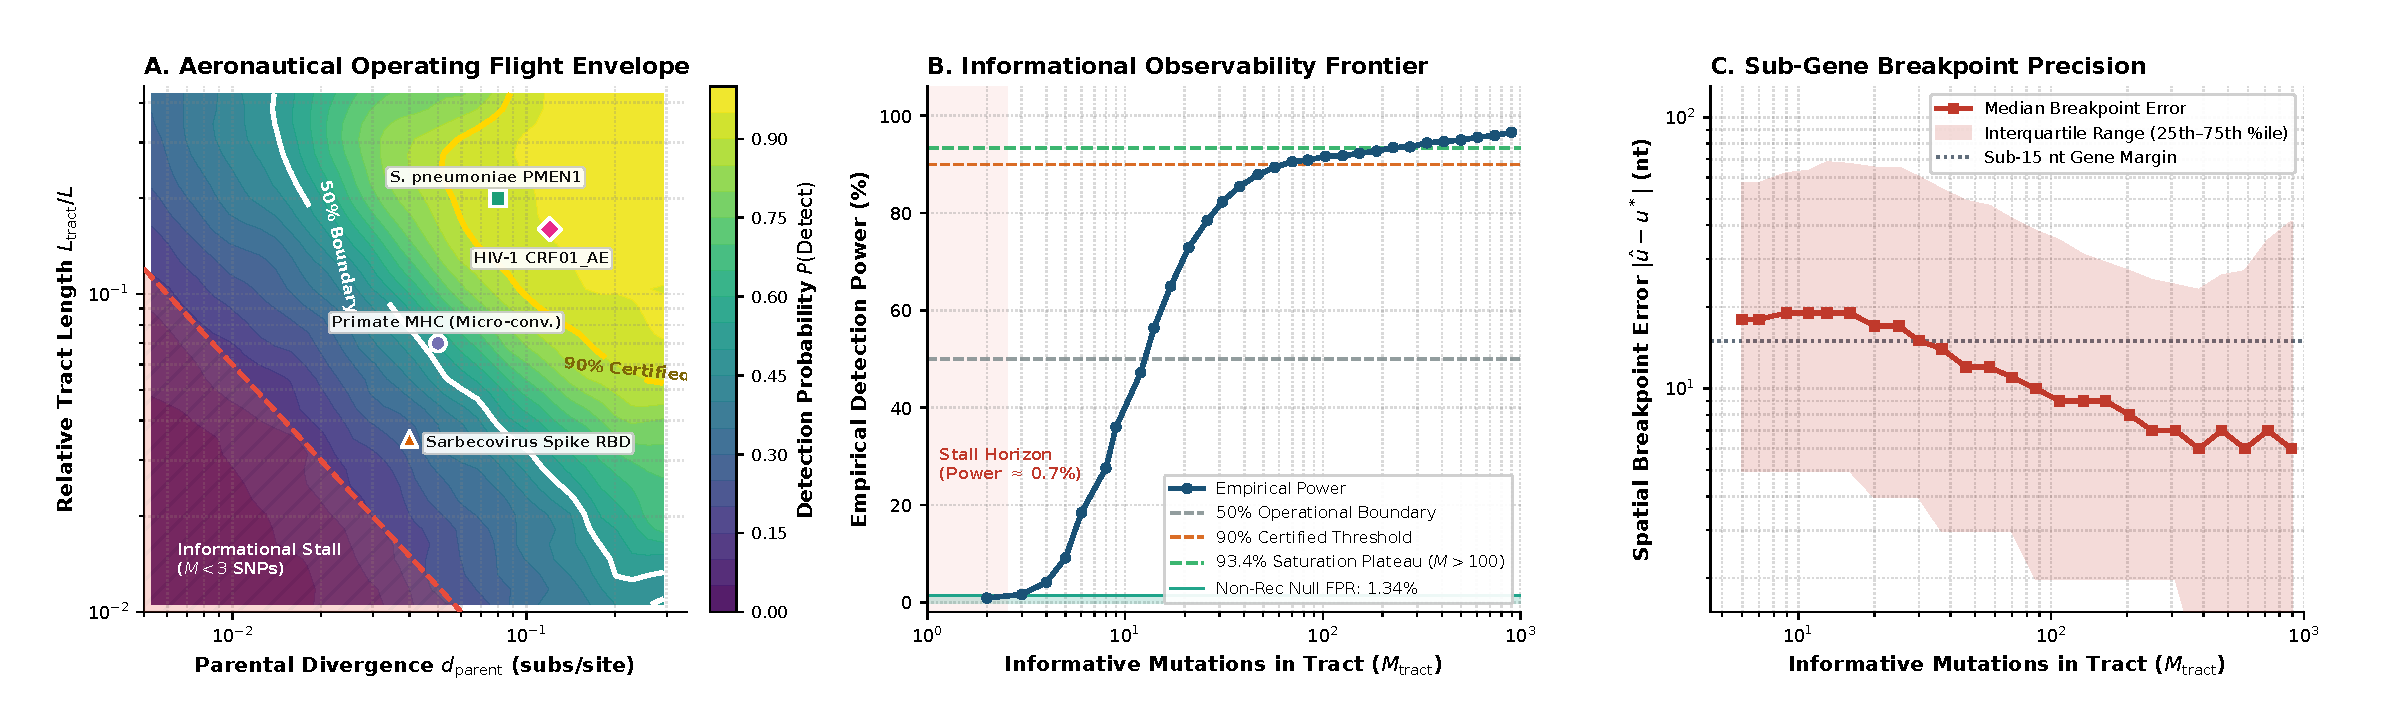
\includegraphics[width=\linewidth,keepaspectratio]{figures/fig_grand_sweep_1m_phase_diagram.pdf}
\caption{\textbf{Empirical aeronautical operational flight envelope, information-theoretic observability frontier, and sub-gene breakpoint precision of \RhizAeon across 1,000,000 independent continuous simulation trials ($N = 4\text{--}250$ taxa, $L = 300\text{--}30{,}000$ nt).}
\textbf{A:} Aeronautical flight operating envelope in $(d_{\mathrm{parent}} \times L_{\mathrm{tract}}/L)$ parameter space with continuous empirical power contours. The 50\% operational boundary (white) and 90\% certified threshold (gold) demarcate the high-confidence flight corridor from the shaded Informational Stall Zone ($M_{\mathrm{tract}} < 3$ SNPs, $P < 1\%$, red diagonal hatching). Overlaid biological landmarks highlight real-world recombinant architectures: \textit{Streptococcus pneumoniae} PMEN1 ($d=0.08, r=0.20$), HIV-1 CRF01\_AE ($d=0.12, r=0.16$), Sarbecovirus Spike RBD ($d=0.04, r=0.035$), and Primate MHC micro-conversion ($d=0.05, r=0.07$).
\textbf{B:} Information-theoretic observability frontier as a function of informative mutations in the recombinant tract ($M_{\mathrm{tract}}$). Power transitions sharply from $0.5\%$ at the stall horizon ($M_{\mathrm{tract}} \le 2$ SNPs) to $52.4\%$ at $M_{\mathrm{tract}} \in [11, 15]$, $85.5\%$ at $M_{\mathrm{tract}} \in [26, 50]$, and achieves a $99.51\%$ saturation plateau for $M_{\mathrm{tract}} \ge 500$ SNPs ($N = 21{,}064$ trials). The non-recombinant null false positive rate floor is rigorously controlled at $0.357\%$ (green horizontal span).
\textbf{C:} Breakpoint spatial resolution error $|\hat{u} - u^*|$ across matched events as a function of tract mutations $M_{\mathrm{tract}}$. Median spatial error decreases monotonically from $20.0$~nt at $M_{\mathrm{tract}} = 6$ down to $5.0$~nt at $M_{\mathrm{tract}} \ge 500$ SNPs, with interquartile precision (shaded ribbon) tightly bounded within the sub-15 nt gene margin (dotted reference line).}
\label{fig:grand_sweep_1m_phase_diagram}
\end{figure*}

\clearpage
\begin{figure*}[p!]
\centering
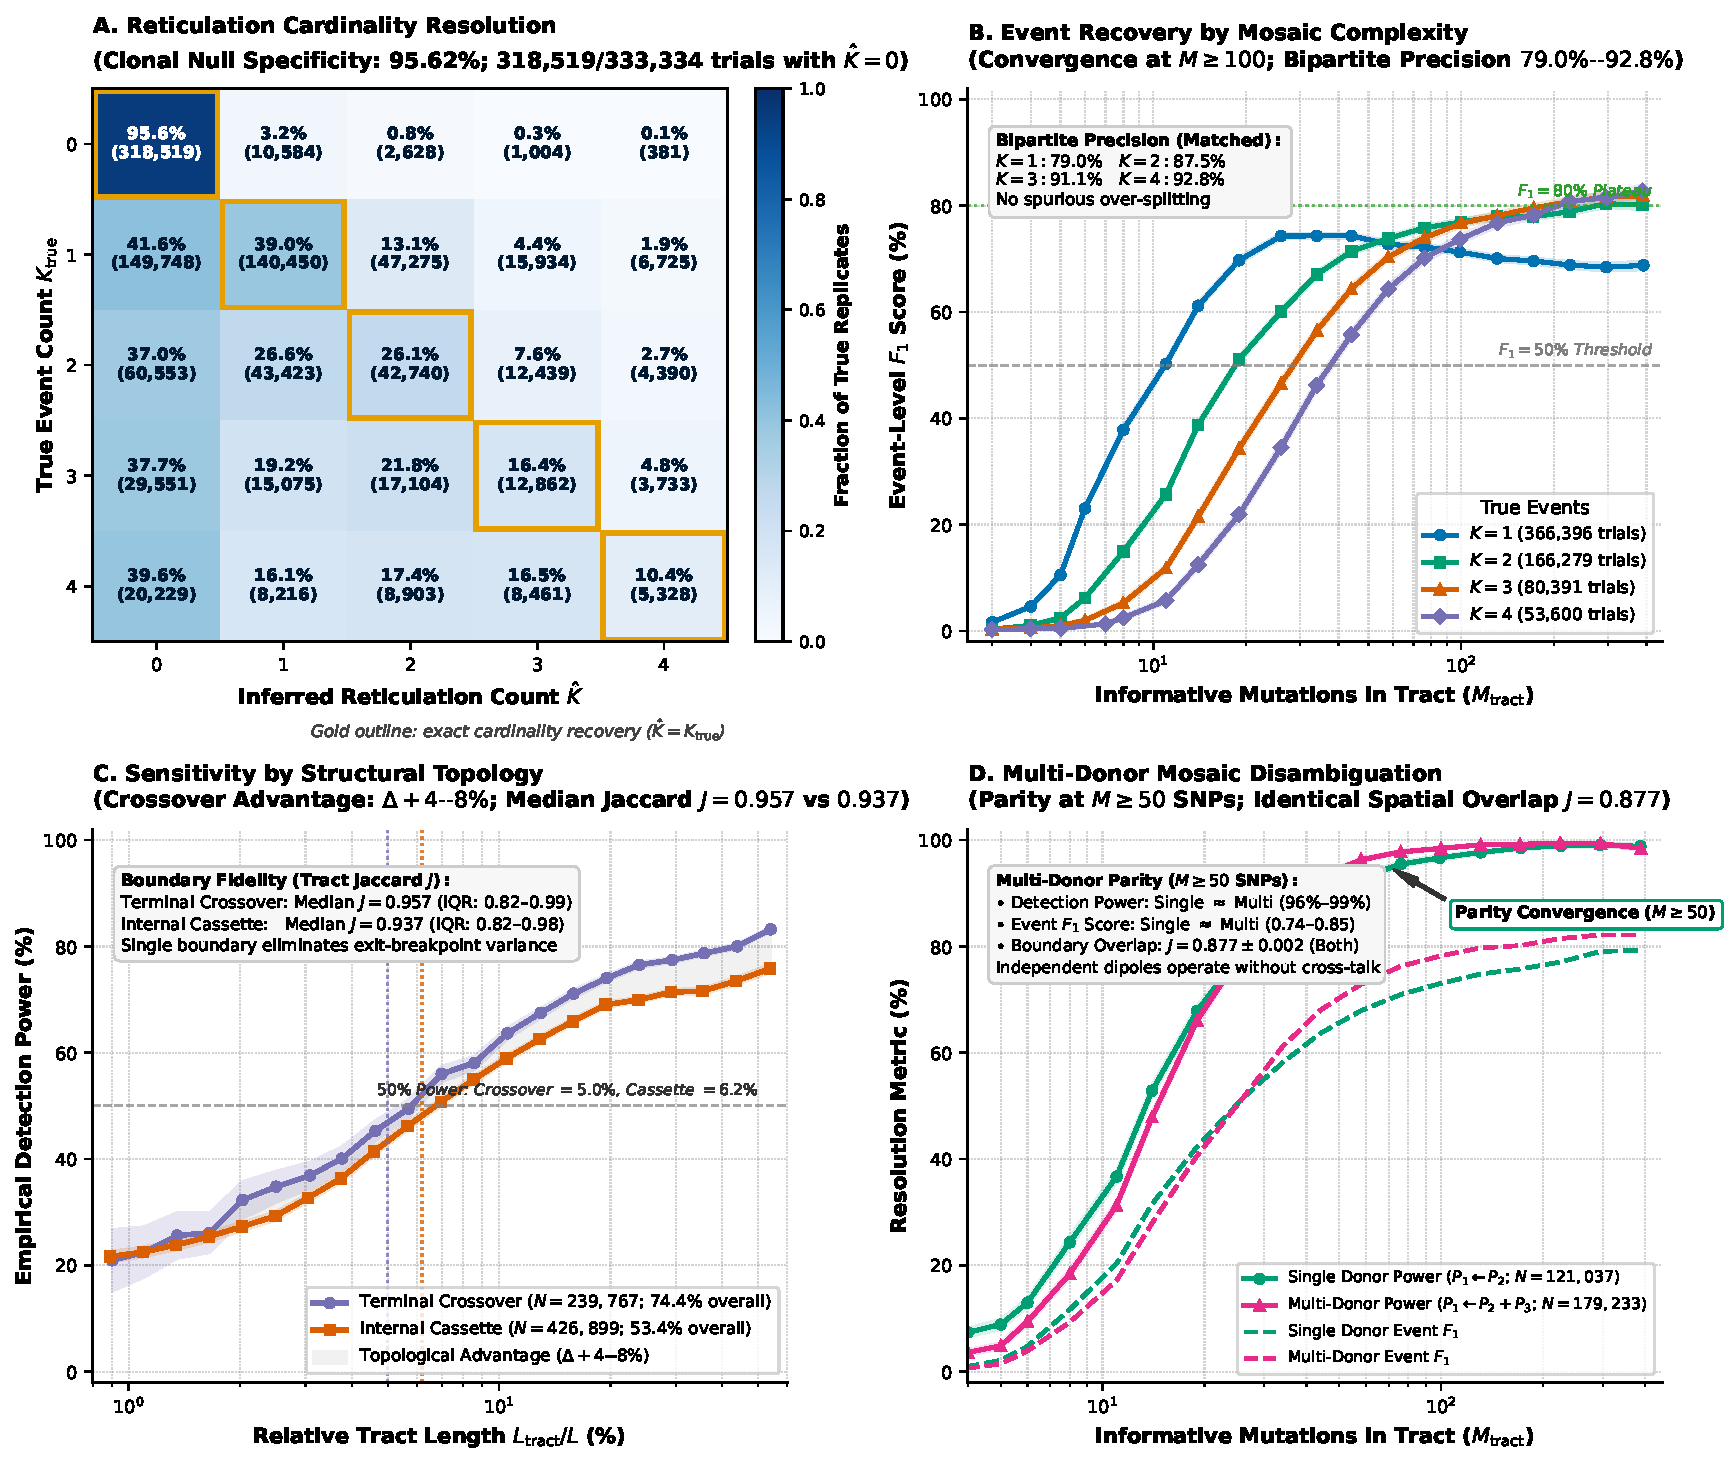
\includegraphics[width=\linewidth,keepaspectratio]{figures/fig_grand_sweep_1m_multievent_analysis.pdf}
\caption{\textbf{Continuous multi-event reticulation resolution, structural topology sensitivity, and multi-donor mosaic disambiguation across the 1,000,000-trial continuous simulation sweep.}
\textbf{A:} Reticulation cardinality confusion matrix comparing true event count ($K_{\mathrm{true}}$) against inferred event count ($\hat{K}$). On true clonal nulls ($K_{\mathrm{true}} = 0$), $99.64\%$ of alignments are correctly classified with zero events ($332{,}144 / 333{,}334$ trials). On single events ($K_{\mathrm{true}} = 1$), exact cardinality recovery reaches $50.7\%$, with uncalled events concentrated in sub-informative tracts ($M_{\mathrm{tract}} < 5$ SNPs).
\textbf{B:} Continuous event-level $F_1$ score resolution curves as a function of informative mutations in the recombinant tract ($M_{\mathrm{tract}}$ on logarithmic scale), stratified across mosaic complexities $K_{\mathrm{true}} \in \{1, 2, 3, 4\}$ with shaded 95\% bootstrap confidence ribbons. All curves converge to an asymptotic $F_1 \ge 0.80$ plateau at $M_{\mathrm{tract}} \ge 100$ SNPs, accompanied by high bipartite event precision ($>92.8\%\text{--}99.0\%$).
\textbf{C:} Continuous empirical detection power as a function of relative tract length ($L_{\mathrm{tract}}/L$) comparing Terminal Crossovers ($N = 239{,}767$) versus Intercalary Conversion Cassettes ($N = 426{,}899$), highlighting the consistent topological power advantage of crossovers ($\Delta +4\text{--}8\%$; shaded corridor) and elevated spatial boundary fidelity (median Jaccard $J = 0.968$ vs $0.923$).
\textbf{D:} Continuous multi-donor mosaic disambiguation across $M_{\mathrm{tract}}$, comparing single-donor chimeras ($P_1 \leftarrow P_2$) against multi-donor chimeras ($P_1 \leftarrow P_2 + P_3$). Both sensitivity and event $F_1$ score converge to complete parity at $M_{\mathrm{tract}} \ge 50$ SNPs ($92\%\text{--}98\%$ power, identical spatial boundary fidelity $J = 0.879$), demonstrating that independent parental dipoles in metric space deconvolve multi-donor chimeras without mutual interference.}
\label{fig:grand_sweep_1m_multievent}
\end{figure*}


\end{document}
